\documentclass[11pt]{article}
\usepackage[T1]{fontenc}
\usepackage{lmodern,amsmath,amssymb,amsthm,mathtools,mathrsfs}
\usepackage[margin=1in]{geometry}
\usepackage{microtype,booktabs,tikz}
\usepackage[hyphens]{url}
\usepackage[colorlinks=true,linkcolor=blue!50!black,citecolor=blue!50!black,urlcolor=blue!50!black]{hyperref}
\hypersetup{pdftitle={Critical honeycomb chords with prescribed boundary endpoints},pdfauthor={OpenAI}}
\ifdefined\pdfinfoomitdate\pdfinfoomitdate=1\fi
\ifdefined\pdftrailerid\pdftrailerid{}\fi
\allowdisplaybreaks[2]
\numberwithin{equation}{section}
\newtheorem{theorem}{Theorem}[section]
\newtheorem{lemma}[theorem]{Lemma}
\newtheorem{proposition}[theorem]{Proposition}
\newtheorem{corollary}[theorem]{Corollary}
\theoremstyle{definition}\newtheorem{definition}[theorem]{Definition}
\theoremstyle{remark}\newtheorem{remark}[theorem]{Remark}
\DeclareMathOperator{\diam}{diam}\DeclareMathOperator{\dist}{dist}
\DeclareMathOperator{\Tr}{Tr}\DeclareMathOperator{\Pf}{Pf}
\DeclareMathOperator{\supp}{supp}\DeclareMathOperator{\Span}{span}
\title{Critical honeycomb chords with prescribed boundary endpoints}
\author{OpenAI}\date{September 26, 2026}
\begin{document}\maketitle
\begin{abstract}
Critical self-avoiding walks between prescribed, macroscopically separated boundary ports of a regular honeycomb hexagon have length $R^{4/3+o(1)}$ in probability, where $R$ is the scale of the hexagon. We prove the corresponding statements for half-plane arches, parallel cuts and nonparallel pure cuts. The half-plane law also has mean length $R^{4/3+o(1)}$. A separate strip argument gives endpoint mean laws on one density-one set of heights and in an aligned, critically weighted mixture of all even heights in a macroscopic interval.
\end{abstract}
\tableofcontents
\section{Introduction}\label{c:introduction}
A boundary-to-boundary walk can be weighted critically without fixing its
length. In that law the separation of the endpoints supplies the spatial
scale. Our question is whether prescribing the terminal boundary point,
rather than summing over an interval, changes the power relating length
to that scale. The distinction is substantial: a macroscopic terminal
interval contains order $R$ ports, and a bound on its total exceptional
mass does not bound the exceptional mass at one specified port.

We use the regular honeycomb lattice, embedded as the centers of the
triangles of an equilateral triangular tiling of side one. Neighboring
centers are joined across a common triangle edge. A \emph{port} is the
midpoint of a boundary edge of a domain made of whole triangles. A path
enters and leaves normally at its ports, visits only centers in the
interior, and visits no center twice. Its length $L(\gamma)$ is the number
of visited centers, and its critical weight is
\[
 w(\gamma)=\kappa^{L(\gamma)},\qquad
 \kappa=(2\cos(\pi/8))^{-1}=(2+\sqrt2)^{-1/2}.
\]
Ports carry no weight. For a domain $D$ and boundary ports $a,b$, set
\[
 K_D(a,b)=\sum_{\gamma:a\to b\text{ in }D}w(\gamma).
\]
Whenever the sum is positive and finite, dividing by it defines the
critical chord law. The path has no other boundary exit. A \emph{pure}
cut follows one of the three tiling-edge directions; its admissible
translates bound whole triangular rows. Distances refer to this fixed
embedding.

\begin{theorem}[Prescribed boundary endpoints]\label{c:main}
Let $D_R$ be convex pure lattice hexagons which, after scaling by $R$,
converge to a regular hexagon. Let $a_R,b_R$ be boundary ports whose
scaled limits are distinct points in the relative interiors of sides.
Then, for every $\varepsilon>0$, the critical chord law satisfies
\[
 \mathbb P_{D_R;a_R,b_R}
 \{R^{4/3-\varepsilon}\le L(\gamma)\le R^{4/3+\varepsilon}\}
 \longrightarrow1.
\]
The same conclusion holds in a full half-plane for prescribed boundary
ports at distance $R$, in a strip of height comparable to $R$ for
one prescribed port on each of the two opposite boundary cuts, at mutual
distance $O(R)$, and in a wedge of angle
$\pi/3$ or $2\pi/3$ formed by two nonparallel pure cuts, with one prescribed port on each ray.
In the wedge, each endpoint has clearance comparable to $R$ from the other cut and
distance $O(R)$ from the apex. Constants are uniform on fixed compact
sets of these nondegenerate scaled geometries. In each case the
normalizing mass is at least $cR^{-5/4}$.
\end{theorem}

The theorem concerns each admissible choice of the two ports. A first
step, proved in Section~\ref{c:window}, fixes the source and sums the
terminal port over a separated macroscopic interval. Its normalizing
mass is of order $R^{-1/4}$. This intermediate law is also useful in its
own right, and remains distinct from the prescribed-endpoint law.

For half-plane arches we additionally prove
$\mathbb E L=R^{4/3+o(1)}$. This requires control of the weighted upper
tail; convergence in probability alone would not imply it. We also record
the terminal-summed mean law from the proof of \cite[Theorem 8.1]{Renewal},
where the gap ranges over $[R,2R]$ and the arch diameter is confined to a
sufficiently large fixed multiple of $R$. For strip
bridges, a second argument proves a mean law uniformly over sublinear
terminal offsets on a single set of heights of natural density one.
It also proves the same mean exponent in the critical mixture of aligned
bridges at all even heights in $[H,2H]$. These mean statements retain their
own height and weighting conventions.

\paragraph{Historical context.}
Nienhuis's analysis of the dilute $O(n)$ model predicted the planar
self-avoiding-walk exponents, including the length--distance power
$4/3$~\cite{Nienhuis1982}. Duminil-Copin and Smirnov proved the honeycomb
connective constant using a local winding relation and a boundary
identity~\cite{DuminilCopinSmirnov2012}. Their mid-edge convention is the
port convention used here. For critical strip mass, Beaton, Bousquet-M\'elou, de Gier,
Duminil-Copin and Guttmann proved decay to zero in their work on surface
adsorption~\cite{BeatonEtAl2014}. Glazman and Manolescu gave a shorter
proof and a logarithmic subsequence bound, and proved boundary two-point
invariance for columnwise rhombic half-planes with angles in
$[\pi/3,2\pi/3]$~\cite{GlazmanManolescu2017}. Krachun and Panagiotis
subsequently proved a polynomial upper bound for strip-crossing mass
and a quantitative sub-ballistic estimate for uniform honeycomb
walks~\cite{KrachunPanagiotis2026}. These results distinguish critical
activity, decay of crossing mass, and length--distance exponents;
the finite inputs below specify the stronger estimates used here.

The irreducible-bridge construction goes back to
Kesten~\cite{Kesten1963}; its honeycomb mid-edge form appears in
\cite[Appendix]{BeatonEtAl2014}. On the square lattice, the infinite
critical law and its relation to strip-spanning laws are developed by
Lawler--Schramm--Werner~\cite[Appendix]{LawlerSchrammWerner2004} and
Dyhr--Gilbert--Kennedy--Lawler--Passon~\cite[Section 2.4]{DyhrEtAl2011}.
Gilbert's appendix records Kennedy's heuristic connecting strip mass
of order $h^{-1/4}$ to an irreducible height tail of order $h^{-3/4}$
and renewal heights of order $n^{4/3}$~\cite[Appendix]{Gilbert2015}.
Here whole irreducible bridges are independent increments; height,
length and lateral displacement within one increment remain dependent.

The quantitative starting point is the sharp finite marked-polygon and
bridge estimates of \cite{UniformMarked}, together with the renewal
estimates of \cite{Renewal}; Section~\ref{c:inputs} states exactly what
we use. These are stronger inputs than the preceding critical and
sub-ballistic results. The terminal-free fixed-height probability law
and the prescribed half-plane arch probability law already appear in
\cite[Propositions 5.7 and 5.8]{Renewal}. We give a different proof of the
latter, through common-level pair renewals and arch-kernel regularity,
and develop the local estimates needed to assemble the prescribed-endpoint
laws in the other geometries. The mean estimates require additional
length-weighted control and retain separate finite inputs.

\paragraph{The three endpoint mechanisms.}
For two ports on one line, grow independent bridge sequences upward from
the two ports and stop at their common renewal levels. Their common
height transform has exponent $1/2$. A separate lateral window estimate
gives $O(m^{-2})$ atoms for the difference after $m$ common blocks. This supplies both regularity
of the arch kernel and control of a long final joining arch; the complete
argument is in Section~\ref{c:same-side}.

For parallel cuts one must match height and lateral displacement at once.
A height-tail bound alone does not pay for one prescribed height.
Section~\ref{c:smoothness-section} bounds all fixed-order differences of
the strip mass, starting from the finite projection representation in
\cite{UniformMarked}. This local regularity gives the one-piece height
atom bound in Section~\ref{c:atoms-section}. Together with two-dimensional
concentration and a sum of heightwise maximal atoms, it pays the parallel
endpoint restriction in Section~\ref{c:parallel-section}.
For nonparallel cuts, small normal prefixes
initially exhaust only a sum over terminal ports. A local visit estimate
and an artificial-arc boundary identity then control the exceptional
mass at the prescribed terminal port. Each case thus pays for its actual
endpoint restriction before dividing by the chord mass;
Section~\ref{c:tilted} completes the nonparallel case.

The means use two further arguments. In Section~\ref{c:mean}, the
calibrated finite estimates of \cite{Calibrated} and their renewal
consequences control marked arms at both ends of an arch. The resulting
length-weighted contributions are summable over arch heights at each
prescribed gap. In Section~\ref{c:pvmeans},
the finite strip moments of \cite{PolynomialVacuum} feed a renewal-reward
identity. A two-bridge boundary comparison controls variation between
terminal ports after averaging over heights, leading to the density-one
and aligned-mixture mean laws rather than an all-height pointwise claim.

\section{Finite estimates and the irreducible law}\label{c:inputs}
We first identify the inputs that do not depend on prescribed endpoints.
A strip of integral height $h$ has physical thickness $dh$, where
$d=\sqrt3/2$. Write $B_h$ for its critical bridge mass from one fixed
bottom port, summed over all compatible top ports, and put $B_0=1$.
A strict bridge stays between its boundary cuts. Its terminal offset lies
on the row-staggered lattice $\mathbb Z+h/2$ in horizontal side units.
There is no translation factor in $B_h$.

\begin{proposition}[Finite boundary and length inputs]\label{c:finite}
The following estimates hold in the port convention above.
\begin{enumerate}
\item For every integer $h\ge0$, $B_h\asymp(1+h)^{-1/4}$.
For all sufficiently large integers $h$, the length-weighted
bridge mass is at most $Ch^{13/12}$, and
$B_h\{L\ge ch^{4/3}\}\ge ch^{-1/4}$.
For every integer $h\ge1$ and every $r\ge0$, the mass of
bridges of diameter exceeding $r$ is at most $C(1+r)^{-1/4}$.
\item In a convex pure domain, the mass from one boundary source of
completed paths of diameter at least $r$ is at most $C(1+r)^{-1/4}$
for $r\ge0$.
For the half-plane arch kernel and integer $l\ge1$,
$K_l\asymp l^{-5/4}$ and $K_{l+1}\le K_l$.
The same monotonicity comparison is valid along one straight side
of a convex pure truncation whenever both compared adjacent ports
remain on that side. Arches of diameter at most
$Al$ retain mass $cl^{-5/4}$ for a fixed $A$.
\item From a prescribed port $a$ with inward pure normal $n$, consider
the terminal line $m\cdot(z-a)=s$, where $m$ is its outward pure unit
normal and the angle between $n$ and $m$ is at most $\pi/3$.
Here $s>0$ is the Euclidean distance from $a$ to the terminal line.
Crossings that stay in the initial half-plane and before the terminal
line until their final exit have mass comparable to $s^{-1/4}$.
For any fixed positive relative tolerance, and all sufficiently large
admissible $s$ with a threshold depending only on that tolerance, the lower
bound can be confined within distance equal to that tolerance times $s$
of the segment $a+[0,s]m$. The corresponding two-cut upper
bound holds without confinement.
\item In a convex pure domain of diameter $O(R)$, the total
length-weighted mass of chords, summed over ordered boundary endpoint
pairs, is at most $R^{25/12+o(1)}$.
\end{enumerate}
\end{proposition}
These are the finite results of \cite[Theorem 1.1, Propositions 7.1, 7.4, 10.1 and Corollary 8.1]{UniformMarked}. The statement records the input
before use; the full analytic and finite geometric proofs are in that
companion. In particular its free-boundary mean is a finite input, not a
consequence of the endpoint theorem here. The disk-transfer construction
\cite[Theorem 1.1]{DiskTransfer} provides an independent fixed-corridor first moment.
We use the specified finite method at each application below; in particular
the logarithmic confinement in the polynomial-vacuum route retains its
own precision.

We use also the local contour identity with phase
$e^{i\sigma W}$, $\sigma=3/8$, where $W$ is total turning.
This is the phase $e^{-5iW/8}$ of the usual observable multiplied by
the terminal tangent relative to the initial direction;
see \cite[Section 2, Lemma 1]{DuminilCopinSmirnov2012}.
At an unvisited center the two outgoing weights sum to the incoming
weight, since $2\kappa\cos(\pi/8)=1$. Prefixes returning to a visited
center cancel in pairs under reversal of their unfinished simple loop:
their turn increments differ by $8\pi/3$, and hence their phases have
opposite signs. Summing over a finite domain gives signed exit mass one.
For a convex domain the real exit coefficients lie in
$[\cos(3\pi/8),1]$. Subtracting the identity in a convex subdomain
bounds the mass of paths lost on restriction by a fixed multiple of the
mass to the newly exposed sides. Exhaustion is justified by the diameter
bound in Proposition~\ref{c:finite}. This is the local winding mechanism
of \cite{DuminilCopinSmirnov2012}; below we explain the additional arc
and spectator constructions when they are used.

An irreducible strict bridge has positive integral height and no
intermediate singly crossed level. Every bridge has a unique ordered
factorization into such pieces. The honeycomb mid-edge version of the
irreducible construction is given in \cite[Appendix]{BeatonEtAl2014}.
Let $p(\gamma)=\kappa^{L(\gamma)}$
on irreducibles from a fixed port. Let $H,Z,L,D$ denote respectively the
height, transverse displacement, length and diameter of one piece.

\begin{proposition}[Renewal inputs]\label{c:renewal}
The mass $p$ is a probability. Successive complete pieces have independent
law $p$, and, for $s>0$,
\[
 \sum_{h\ge0}B_he^{-sh}=
 (1-\mathbb E_p e^{-sH})^{-1}\asymp s^{-3/4}\quad(s\downarrow0).
\]
Moreover,
\[
 p(H>x)+p(D>x)\le Cx^{-3/4},\quad
 \mathbb E_p[L;H\le x]\le x^{7/12+o(1)},
\]
\[
 p(L>n)\le n^{-9/16+o(1)},\qquad
 1-\mathbb E_p e^{-uL}=u^{9/16+o(1)}.
\]
Almost surely, for independent pieces, their first $k$ heights and lengths
sum respectively to $k^{4/3+o(1)}$ and $k^{16/9+o(1)}$, and their
diameters sum to at most $k^{4/3+o(1)}$.
\end{proposition}
The proofs and the full joint-law conventions are
\cite[Propositions 2.2, 2.4, Remark 2.5 and Lemma 2.6]{Renewal}. Only the independent \emph{pieces}
are asserted here; their coordinates are not independent. $B_h$ is a
renewal occurrence mass, not a probability conditioned on a future height.
No estimate in this proposition conditions a piece on its length.

Throughout, $f(R)=R^{a+o(1)}$ means
$R^{a-\varepsilon}\le f(R)\le R^{a+\varepsilon}$ for every fixed
$\varepsilon>0$ at all sufficiently large scales, with fixed geometric
parameters chosen first. A one-sided use retains just the corresponding
inequality. All suprema of atoms are on their actual support lattice;
off-lattice probabilities are zero.

\section{A prescribed source and a terminal interval}\label{c:window}
Prescribing one endpoint and summing the other over a separated interval
gives normalizing mass of order $R^{-1/4}$. We first establish this
normalization by constructing interior connectors. We then prove the
bridge and attachment estimates that transfer the length law to these
chords. The attachment estimates will also be used for nonparallel cuts
in Section~\ref{c:tilted}.

\subsection{Interior connectors}

\begin{proposition}[Interior connectors]\label{c:connectors}
For two macroscopically separated side-interior ports in the hexagons of
Theorem~\ref{c:main}, the critical mass of connecting paths inside the
hexagon is at least $cR^{-5/4}$. The same bound holds in a parallel strip
of thickness comparable to $R$, with one port on each opposite cut and
displacement $O(R)$, and in compact nondegenerate wedge geometries with
one port on each ray, as in Theorem~\ref{c:main}. The constants are uniform
on fixed compact sets of these scaled configurations.
\end{proposition}
\begin{proof}
We adapt the cut-averaging construction in the proof of
\cite[Proposition 10.2]{UniformMarked}, placing the routes in the interior
rather than the exterior. The geometric choices below ensure that the
decomposition can be recovered for two different lists of cuts.

\paragraph{Routes and junction cuts.}
Work first in a hexagon and scale distances by $R$. Start with short
segments in the inward normals at the two ports. Continue by disjoint
simple arcs in the open interior to two parallel lanes in a free interior
ball, preserving their cyclic order. The lanes approach one common pure
transverse line from the same side. Their separation is a small fixed
positive number, so a completing arch of diameter at most a fixed
multiple of that separation fits in the free half-ball beyond the line.
Keep that half-ball disjoint from all nonincident route portions.

Approximate the arcs by finitely many segments in pure normal directions,
retaining the initial and terminal straight portions and making successive
direction changes at most $\pi/3$. One can do this by alternating the two
adjacent pure directions spanning each smooth tangent, with a short step
in their common direction at a sector transition. A sufficiently fine
fixed mesh preserves separation of nonlocal portions; on nearby portions,
positive projection in a common direction preserves simplicity. Every
segment has length a fixed positive multiple of $R$.

Index a branch's segments by their guiding directions $n_j$. The cut at
the end of segment $j$ has normal $n_j$, the \emph{arriving} direction.
The next leg starts with inward normal $n_j$ and travels toward a cut
with outward normal $n_{j+1}$. Proposition~\ref{c:finite}(iii) therefore
keeps the incoming leg before the junction cut and the outgoing leg
after it. Restrict each leg to a sufficiently narrow corridor about its
segment. Each junction has its own small crossing neighborhood, avoided
by all nonincident route portions. This is a local requirement: those
portions need not avoid the entire infinite line of the cut.

The geometric choices have positive clearances. They persist in a
neighborhood of the scaled endpoint data, including the small support
perturbations allowed in Theorem~\ref{c:main}. Compactness gives uniform
choices of the number of segments and their relative tolerances.

\paragraph{One list and two lists of levels.}
Vary each junction cut in a fixed small window of admissible levels of
width comparable to $R$. Choose the windows so that all corridors and
stage orders just described persist for every list. The terminal level
is shared by the two branches; all other levels vary independently.
If there are $k$ legs in total, the set $\Lambda_R$ of level lists is
thus a product of $k-2$ ordinary windows and one shared terminal window.
Give it the uniform product probability measure.

For a list $\lambda$, let $I_\lambda(\gamma)$ indicate that the chord
splits into the confined legs and the completing arch at these cuts.
The splitting is unique. At each isolated junction the two incident
pieces meet the cut once and occupy its opposite half-planes; all other
pieces avoid that crossing neighborhood. Put
\[
 F_R(\gamma)=\frac1{|\Lambda_R|}\sum_{\lambda\in\Lambda_R}I_\lambda(\gamma),
 \qquad
 \int G\,d\mu=\sum_{\gamma:a\to b}\kappa^{L(\gamma)}G(\gamma).
\]
Multiplication of the $k$ point-to-line lower bounds and the confined
arch lower bound gives
\[
 \int F_R\,d\mu\ge cR^{-k/4-5/4}.
\]

For two lists, split each branch at both crossings in each junction
neighborhood. The two crossings occur in their normal-level order:
the incoming portions start below both levels, and the outgoing
portions end above both. The intervening portion is consequently a
strict bridge of the level difference. The portions between successive
neighborhoods still have separation comparable to $R$ and cost
$O(R^{-1/4})$ each. There are $k$ such long portions. Beyond the later
shared terminal line the remaining arch costs $O(R^{-5/4})$.

For two independent uniform levels $u,u'$ in a window of order $R$,
\[
 \mathbb E(1+|u-u'|)^{-\alpha}\le C_\alpha R^{-\alpha}
 \qquad(0<\alpha<1).
\]
Every ordinary junction gives one difference bridge and uses this bound
with $\alpha=1/4$. The shared terminal level gives two difference
bridges, one on each branch, and uses $\alpha=1/2$. Ties are included
by the convention $B_0=1$. Averaging the joint mass therefore gives
\[
 \int F_R^2\,d\mu
 \le C\underbrace{R^{-k/4}}_{\text{long portions}}
       \underbrace{R^{-(k-2)/4}R^{-1/2}}_{\text{difference bridges}}
       \underbrace{R^{-5/4}}_{\text{terminal arch}}
 =CR^{-2k/4-5/4}.
\]
Cauchy--Schwarz now yields
\[
 \mu(F_R>0)\ge
 \frac{(\int F_R\,d\mu)^2}{\int F_R^2\,d\mu}
 \ge cR^{-5/4}.
\]

For a wedge, add distant pure cuts at distance $AR$ from the endpoints,
with $A$ fixed and sufficiently large. The endpoint clearances to the
opposite supports permit initial inward segments of length $cR$.
The resulting bounded convex patch contains an interior ball of radius
$c'R$ accessible by the two separated routes above. After scaling, these
choices persist on a neighborhood of each nondegenerate configuration;
a finite cover of the compact family gives uniform clearances. The
constructed paths stay in the full wedge. A parallel strip admits the
same bounded-patch construction. This proves all the stated cases.
\end{proof}

\begin{theorem}[A source and a macroscopic terminal interval]\label{c:window-law}
In the hexagons of Theorem~\ref{c:main}, fix a source port tending after
scaling to a side-interior point. Let the terminal ports form a
macroscopic interval converging to a compact side-interior interval at
positive distance from the source limit. Under critical weights,
normalized over those chords, length is $R^{4/3+o(1)}$ in probability.
The same holds when the source is summed over a separated macroscopic
side-interior interval. For each fixed source the normalizer is
comparable to $R^{-1/4}$.
\end{theorem}

The diameter bound gives the upper normalization, and summing
Proposition~\ref{c:connectors} over order-$R$ terminal ports gives the
lower one. We prepare the length estimates next; the proof of the theorem
is completed at the end of this section.

\subsection{Bridge length and displacement windows}

\begin{lemma}[Fixed-height bridge length]\label{c:fixed-height-window}
Under critical weights on strict bridges of integral height $h$, with
one initial port fixed and the terminal port summed, for every $\delta>0$,
\[
 \Pr\{h^{4/3-\delta}\le L\le h^{4/3+\delta}\}\longrightarrow1.
\]
The same conclusion holds after any restriction retaining a fixed positive
fraction of $B_h$.
\end{lemma}
The fixed-height conclusion also appears in
\cite[Proposition 5.7]{Renewal}. We give the argument from the finite
and renewal inputs selected in Section~\ref{c:inputs}.
\begin{proof}
It suffices to treat $0<\delta<1$. The upper length tail follows from
$B_h^{-1}\sum Lw\le Ch^{4/3}$. For the lower tail, first obtain a
height window under the one-piece law $p$. There are fixed $M,A>1$ with
\begin{equation}\label{c:one-piece-height-window}
 p\{x\le H\le Mx,\ D\le Ax\}\ge cx^{-3/4}
\end{equation}
for all sufficiently large $x$. Indeed
$\mathbb E_p[1-e^{-H/(Kx)}]\asymp(Kx)^{-3/4}$, whereas the contribution
from $H\le x$ is $O(x^{-3/4}/K)$ and that from $H>Mx$ is
$O((Mx)^{-3/4})$. Choose first $K$, then $M$, sufficiently large.
Finally the diameter tail permits $A\ge M$ large enough to retain the
lower bound.

This window gives the concentration estimate
\begin{equation}\label{c:height-sum-atom}
 \sup_j\Pr(H_1+\cdots+H_k=j)\le Ck^{-4/3}.
\end{equation}
To see this, symmetrize the characteristic function using an independent
copy of $H$ that is bounded with positive probability. In
\eqref{c:one-piece-height-window}, take $x$ to be a sufficiently small
fixed multiple of $|\theta|^{-1}$. The cosine deficit on that event is
bounded below, so the squared modulus loses at least
$c|\theta|^{3/4}$ near zero. The modulus has only finitely many peaks
on the lattice torus, repeats the same bound near each, and is bounded
away from one on the remaining compact set. Fourier inversion proves
\eqref{c:height-sum-atom}.

For $k\ge2$, split the pieces into comparable independent halves.
If their total height is $h$, one half has height at least $h/2$, at
cost at most $Ckh^{-3/4}$ by the tail and truncated first moment.
The other half matches a height atom at cost $Ck^{-4/3}$. The case
$k=1$ costs at most $Ch^{-3/4}$. Hence, for fixed $\eta>0$,
\[
 \sum_{1\le k\le h^{3/4-\eta}}
 \Pr\Bigl\{\sum_{j\le k}H_j=h\Bigr\}
 \le Ch^{-3/4}\left(1+
       \sum_{2\le k\le h^{3/4-\eta}}k^{-1/3}\right)
 =o(B_h).
\]
For the remaining counts put $t=h^{4/3-\delta}$. Exponential Markov
and the length deficit give
\[
 \Pr\Bigl\{\sum_{j\le k}L_j<t\Bigr\}
 \le e(\mathbb E_p e^{-L/t})^k
 \le e\exp\{-k t^{-9/16+o(1)}\}.
\]
Choose $\eta<9\delta/16$. Summing this geometric bound over
$k>h^{3/4-\eta}$ is stretched-exponentially small. The renewal
factorization proves the lower length tail after division by $B_h$.
Dividing instead by any fixed positive fraction of $B_h$ preserves
both negligible exceptional masses.
\end{proof}

We next arrange a displacement that points inward at both chord ends.
This is needed when a translated chord is attached back to its original
supports. Distances in the following geometric statement are physical;
the bridge height $h$ is still in row units.

\begin{lemma}[Positive projections at two supports]\label{c:positive-projection}
Let $n,m$ be pure unit normals with $m\ne-n$. There are constants
$b,B,A,c_0>0$ such that, for every fixed $\delta>0$ and all sufficiently
large integral $h$, the mass of strict $n$-bridges from a fixed port
with endpoint displacement $v$, restricted by
\[
 bh\le m\cdot v\le Bh,\qquad D\le Ah,\qquad
 h^{4/3-\delta}\le L\le h^{4/3+\delta},
\]
is at least $c_0h^{-1/4}$. The constants may depend on $n,m$ but not
on $\delta$; the threshold may depend on $\delta$.
\end{lemma}
\begin{proof}
If $m\cdot n>0$, use a sufficiently narrow straight channel along $n$.
The remaining case is an angle of $2\pi/3$. Let $n'$ be the pure normal
at angle $\pi/3$ to both, and put $T=dh$. First travel to an $n'$-normal
cut at distance near $3T/2$ from the source, then travel in direction
$n$ to the top cut of the $n$-strip. Proposition~\ref{c:finite}(iii)
guides the first leg along $n'$, even though its initial inward normal
is $n$. At the intermediate position, both the $n$- and $m$-projections
are near $3T/4$. The final leg advances about $T/4$ along $n$, leaving
$m$-projection near $5T/8$. Small fixed tolerances keep both legs
between the $n$-strip boundaries, on opposite sides of the intermediate
cut, and within diameter $O(h)$.

Average that cut over a small window of order $h$. For one cut the two
legs have product mass at least $ch^{-1/2}$. For two cuts, recovery in
level order gives two long turned crossings and a difference bridge;
the averaged joint mass is at most $Ch^{-3/4}$. Cauchy--Schwarz gives
mass at least $ch^{-1/4}$ with the stated geometric restrictions.
In both angular cases this is a fixed fraction of $B_h$.
Lemma~\ref{c:fixed-height-window}, used with slightly smaller exponent
slack, removes the atypical lengths without changing the lower constant
for all sufficiently large $h$.
\end{proof}

\subsection{The cost of two translation choices}

Fix pure normals $n,m$ with $m\ne-n$. For a lattice translation $z$
with $n\cdot z>0$, let $D_n(z)$ be the critical mass of strict
$n$-bridges between the prescribed positions separated by $z$.
For $n\cdot z<0$, set $D_n(z)=D_n(-z)$; thus the bridge is always
oriented in increasing $n$-level order. At zero height set
$D_n(0)=1$ and $D_n(z)=0$ for nonzero $z$ with $n\cdot z=0$.

\begin{lemma}[Mixed displacement estimate]\label{c:mixed-displacement}
For every fixed $C_0<\infty$ there is $C<\infty$ such that, for $s\ge1$,
\begin{equation}\label{c:mixed-displacement-bound}
 \sum_{|z|\le C_0s}D_n(z)(1+|m\cdot z|)^{-1/4}\le Cs^{1/2}.
\end{equation}
If $Y$ is the $m$-projection of one $n$-directed irreducible displacement,
then its independent sums also satisfy
\begin{equation}\label{c:projected-concentration}
 \sup_y\Pr\Bigl\{\sum_{j\le k}Y_j=y\Bigr\}\le Ck^{-4/3},
 \qquad
 \sup_w\mathbb E\Bigl(1+\Bigl|w+\sum_{j\le k}Y_j\Bigr|\Bigr)^{-1/4}
 \le Ck^{-1/3}.
\end{equation}
\end{lemma}
\begin{proof}
The height-and-diameter window \eqref{c:one-piece-height-window} and
lateral reflection symmetry imply, for fixed $B>b>0$,
\[
 p\{bx\le |Y|\le Bx\}\ge cx^{-3/4}.
\]
Indeed the two reflected displacements have $m$-projections whose sum
is $2(m\cdot n)dH$. Since $m\cdot n\ne0$, at least one has magnitude
comparable to $H$, while the diameter cutoff bounds both from above.
The same symmetrization and Fourier argument as for
\eqref{c:height-sum-atom} gives the first bound in
\eqref{c:projected-concentration} on the projection's actual lattice.
For the second, sum this atom bound with weight $(1+|y|)^{-1/4}$
over $|y|\le k^{4/3}$, and bound the weight outside by $k^{-1/3}$.
This is uniform over translated lattices and the shift $w$.

It suffices to sum over $n\cdot z\ge0$ in
\eqref{c:mixed-displacement-bound}. Use renewal factorization, splitting
$k\ge2$ pieces into comparable halves. The displacement restriction
implies total height at most $C_1s$. Height damping bounds this event
on the first half by
\[
 C\exp\{-ck/s^{3/4}\}.
\]
Conditioning on that half, the second bound in
\eqref{c:projected-concentration} applies to the other half, with a
shift given by the first half's projection. Thus the sum is at most
\[
 C+C\sum_{k\ge2}e^{-ck/s^{3/4}}k^{-1/3}\le Cs^{1/2}.
\]
The constant covers one piece and the zero-height match. No coordinates
within one piece have been made independent.
\end{proof}

\subsection{Recoverable attachments}

Consider the two inward support normals $n,m$ at a source $a$ and a
terminal interval whose distances from $a$ are comparable to $R$.
When the supports differ, assume the endpoints have order-$R$ clearance
to the other support, as in the geometries above. We treat $m\ne-n$;
opposite supports will use Lemma~\ref{c:fixed-height-window} directly.
For identical supports their common half-plane replaces the two-cut
domain.

Choose a small fixed $c>0$ and a large scale $s\le cR$. Translate an
input chord by a lattice vector $v$ with $|v|\le Cs$ and both
\[
 g_1=n\cdot v/d,\qquad g_2=m\cdot v/d
\]
between fixed positive multiples of $s$. Attach a height-$g_i$ bridge
from each translated endpoint out to its original support. Restrict the
two bridges to diameter at most $C's$ and length between
$s^{4/3-\delta}$ and $s^{4/3+\delta}$. Such restrictions retain fixed
fractions of the available bridge mass, by the preceding lemmas and the
diameter tail. The branches stay in separated endpoint neighborhoods.
They avoid the translated chord by its supports, and, for distinct
supports, each stays beyond the translated support at the other end
by endpoint clearance and the small choice of $c$.

\begin{proposition}[Attachment moments]\label{c:attachment-proposition}
Let $\mathcal E$ be an event of input chords from $a$ to the stated
terminal interval, of critical mass $E$. The fixed-source attachment
construction just described has a translation count $N_s$ on output
chords and critical output measure $\mu_a$ such that
\begin{equation}\label{c:attachment-moments}
 \int N_s\,d\mu_a\ge cs^{1/2}E,
 \qquad
 \int N_s^2\,d\mu_a\le CsR^{-1/4}.
\end{equation}
Here the side-1 outer landing is exactly $a$; the side-2 outer landing
is free on its support. The estimate applies also to input chords in
the full two-cut domain, without a diameter bound.

If the input chords lie in a convex pure domain of diameter $O(R)$,
there is also a construction at scale $s=cR$ with both outer landings
free, all outputs in one convex pure domain of diameter $O(R)$, and
\begin{equation}\label{c:free-attachment-moments}
 \int N_R^{\rm free}\,d\mu_{\rm free}\ge cR^{3/2}E,
 \qquad
 \int(N_R^{\rm free})^2\,d\mu_{\rm free}\le CR^{7/4}.
\end{equation}
The measure $\mu_{\rm free}$ sums critical weights over ordered output
endpoint pairs. In both constructions output length is the input length
plus the two attached lengths. Constants are uniform for fixed compact
endpoint geometries and independent of the fixed length slack $\delta$;
the required lower threshold for $s$ may depend on $\delta$.
\end{proposition}
\begin{proof}
For fixed source $a$, reverse the side-1 bridge: it starts at $a$ and
must have displacement exactly $v$. Let $\mathcal V_s$ be all translations
in the size and positive-projection ranges above, with ranges wide enough
to include those in Lemma~\ref{c:positive-projection}. At each of order
$s$ heights, that lemma supplies restricted bridge mass at least
$c_0s^{-1/4}$ after summing over its allowed displacements. Thus the
total side-1 mass summed over $v$ is at least $cs^{3/4}$. Side 2 has
its outer landing free and supplies at least $cs^{-1/4}$ for each $v$.

Let $\mathcal A_v(\mathcal E)$ be the set of output chords obtained with
translation $v$, and define
\[
 N_s(\Gamma)=\sum_{v\in\mathcal V_s}
              \mathbf1_{\{\Gamma\in\mathcal A_v(\mathcal E)\}}.
\]
For a fixed $v$ the output determines its decomposition: the crossings
of the two translated supports separate the outer bridges from the
central translated chord. On identical supports there are two crossings,
localized near the two respective endpoints. Critical weights multiply,
since the joining ports have no weight. This proves the first inequality
in \eqref{c:attachment-moments}.

\paragraph{Recovering two translations.}
For $v,v'$, order the two crossings on each branch by that branch's
inward normal height. Their orders may disagree between the two ends.
Nevertheless both side-1 crossings occur before either side-2 crossing
along the output chord: the outer prefixes and suffixes are localized
in the two disjoint endpoint neighborhoods. Split into five portions:
the side-1 outer bridge, its difference bridge, a central chord, the
side-2 difference bridge, and the side-2 outer bridge.

The central portion is between the two innermost crossings. It stays
inside both corresponding supports, because each construction remains
beyond its own translated support after crossing, except for its
localized branch at the other end when the supports coincide. Those
other-end branches lie outside the central portion. Its initial point
is prescribed once the two translations are fixed, its terminal point
is free, and their separation is of order $R$. Dropping all other
conditions bounds its mass by $CR^{-1/4}$.

Put $z=v'-v$. The side-1 difference has prescribed displacement $z$
in one of its two orientations and costs $D_n(z)$. On side 2 the outer
crossing is free, so the difference costs at most
$C(1+|m\cdot z|)^{-1/4}$. If the side-1 heights tie, its unique local
crossing forces $v=v'$; thus the zero-height convention for $D_n$ is
the correct one. The side-2 outer bridge costs $Cs^{-1/4}$. Finally,
if $v_{\rm out}$ is the earlier side-1 translation, the side-1 outer
bridge costs $D_n(v_{\rm out})$, with
\[
 \sum_{v_{\rm out}\in\mathcal V_s}D_n(v_{\rm out})
 \le C\sum_{h\le Cs}B_h\le Cs^{3/4}.
\]
These upper bounds may be multiplied after dropping avoidance constraints
between the five portions. Lemma~\ref{c:mixed-displacement} sums the two
difference factors. The complete accounting is
\[
 \int N_s^2\,d\mu_a
 \le C\underbrace{s^{3/4}}_{\substack{\text{side-1}\\\text{outer sum}}}
       \qquad\underbrace{s^{1/2}}_{\substack{\text{two}\\\text{differences}}}
       \qquad\underbrace{R^{-1/4}}_{\substack{\text{central}\\\text{chord}}}
       \qquad\underbrace{s^{-1/4}}_{\substack{\text{side-2}\\\text{outer}}}
 =CsR^{-1/4}.
\]
The argument used the two supports and endpoint clearance, not a bound
on the diameter of the input chord.

\paragraph{Both outer landings free.}
Take $s=cR$ and sum over order $R^2$ translations in a fixed positive
sector. Both outer bridges now have one free endpoint, so the first
moment is at least $cR^2R^{-1/2}E$. The same two-list recovery keeps
the inner side-1 crossing prescribed. Its outer bridge is now summed
over its original-support landing, replacing the previous outer sum by
$O(R^2R^{-1/4})$. The other three factors are unchanged. Thus
\[
 \int(N_R^{\rm free})^2\,d\mu_{\rm free}
 \le CR^{2-1/4}R^{1/2}R^{-1/4}R^{-1/4}=CR^{7/4}.
\]
The localized attachments and $O(R)$ translations of bounded input
chords all fit in one convex pure truncation of diameter $O(R)$.
This proves \eqref{c:free-attachment-moments}.
\end{proof}

\subsection{Proof of the interval length law}

\begin{proof}[Proof of Theorem~\ref{c:window-law}]
It suffices to prove the length bounds for $0<\epsilon<1$.
The normalizing mass is comparable to $R^{-1/4}$, as shown above.
If the two inward normals are opposite, the chords are a restriction
of height-$h$ bridges with $h\asymp R$, retaining a fixed fraction of
$B_h$. Lemma~\ref{c:fixed-height-window} gives the result. Otherwise
use Proposition~\ref{c:attachment-proposition}.

For an input event of mass $E=p_0R^{-1/4}$, its fixed-source outputs
have mass at least
\[
 \mu_a(N_s>0)\ge
 \frac{(\int N_s\,d\mu_a)^2}{\int N_s^2\,d\mu_a}
 \ge cp_0^2R^{-1/4}.
\]
All these outputs have endpoints separated by order $R$, so their
total mass is at most $CR^{-1/4}$ by the diameter bound.

Apply this to input lengths below $R^{4/3-\epsilon}$. Choose any fixed
number $M$ of distinct exponents $\gamma_j$ in
$(1-\epsilon/3,1)$ and use $s_j=R^{\gamma_j}$. Choose $\delta>0$
small enough that the $M$ output length windows are disjoint and each
attached length dominates the original short input. The lower mass
constant is independent of this fixed $\delta$. Consequently
$Mcp_0^2\le C+o(1)$. Let $R\to\infty$ first and then $M\to\infty$.
This proves $p_0\to0$ for the short-length event.

For input lengths above $R^{4/3+\epsilon}$, use both free landings.
Equation~\eqref{c:free-attachment-moments} gives output mass at least
\[
 c\frac{R^3E^2}{R^{7/4}}=cp_0^2R^{3/4}.
\]
Every output remains long. Proposition~\ref{c:finite}(iv) bounds its
mass in the encompassing convex domain by
\[
 R^{-4/3-\epsilon}R^{25/12+o(1)}=o(R^{3/4}).
\]
Thus $p_0\to0$ also for the long-length event. All bounds are uniform
over the permitted source interval. Summing exceptional masses and
normalizers over that interval proves the source-summed assertion.
\end{proof}

\section{Two prescribed ports on one line}\label{c:same-side}
Fix two boundary ports at distance $l$ in a half-plane. The following
argument grows independent prefixes from them, then joins those prefixes
above their next common renewal level. The joining kernel must become
insensitive to a sublinear change of its endpoint separation. We prove
that regularity here, using the same pair process that controls the
length of the joining path.
The half-plane probability conclusion below is also established in
\cite[Proposition~5.8]{Renewal}. Here the common-level argument supplies
local regularity of the arch kernel as well as the length law, which we
then transfer to the same-side hexagon law.

\begin{theorem}[Same-side probability law]\label{c:same-side-law}
Under the critical half-plane law $w(\gamma)/K_l$, for every
$\varepsilon>0$,
\[
 \mathbb P\{l^{4/3-\varepsilon}\le L(\gamma)
                   \le l^{4/3+\varepsilon}\}\longrightarrow1.
\]
The same conclusion holds in the hexagons of Theorem~\ref{c:main} when both scaled
endpoints converge to distinct points in one side interior.
\end{theorem}
\subsection{Common blocks and lateral concentration}
We use the intersection-renewal construction discussed in
\cite[Section~1.1]{AlexanderBerger2016}, proving the required identities
directly. Distances along the base are physical distances, with port
spacing one; heights are in row units. Run two independent sequences of
upward irreducibles of law $p$, translating each new piece to the current
endpoint. Stop at their next common positive renewal height. Let $r$ be
the resulting mass on finite pairs of terminating sequences, initially
possibly a subprobability, and let $T$ be their common height.

A pair block contains one complete bridge segment from each sequence,
possibly made of several irreducibles. Let $D_*$ be the maximum of the
diameters of these two complete segments, and let $Y$ be the second
segment's lateral displacement minus the first's. In particular,
$|Y|\le2D_*$. Successive common blocks regenerate independently: testing
a prescribed pair of terminating sequences uses only the pieces up to
their termination.

\begin{lemma}[Common-block estimates]\label{c:pair-block-estimates}
The pair-block mass $r$ is a probability. For $x\ge1$,
\[
 r(T>x)+r(D_*>x)\le Cx^{-1/2}.
\]
If $Y^{(m)}$ is the sum of the lateral differences of $m$ independent
pair blocks, then
\[
 \sup_j\Pr(Y^{(m)}=j)\le Cm^{-2}\qquad(m\ge1).
\]
\end{lemma}
\begin{proof}
The common renewal masses are $B_h^2$, so
\[
 C(s)=\sum_{h\ge0}e^{-s h}B_h^2=(1-\hat r(s))^{-1}\asymp s^{-1/2},\qquad
 \hat r(s)=\sum r e^{-sT}.
\]
Sending $s$ to zero shows that $r$ has total mass one, and
$1-\hat r(s)\asymp s^{1/2}$ gives the height-tail estimate.
For the diameter estimate use \(s=D/x\) with \(D\) large fixed in \(C(s)\). The fraction containing a pair-block with \(D_*>x\) is at most \(C x^{-1/4}s^{-3/4}/C(s)<1/2\), using the diameter estimate on one total bridge and the ordinary \(B_h\) bound on the other. More explicitly put $d_s=1-\hat r(s)$ and $q_s=\mathbb E_r[e^{-sT};D_*>x]$. The fraction of terminated lists containing such a block is $q_s/(d_s+q_s)$, so the preceding bound below $1/2$ gives $q_s\le d_s=O(x^{-1/2})$; remove the discount below height \(x\), and above use the height tail from \(1-\hat r(s)\).



\paragraph{A lateral fluctuation in one common block.}
The common-height transform identifies the time scale. We next show that
the transverse difference fluctuates on the same scale; otherwise it
could not smooth a prescribed separation. We claim there are fixed \(D_1>D_0>0\) with
\[
 r(D_0 x\le |Y|\le D_1 x)\ge c x^{-1/2}
\]
for large \(x\). At every large height \(h\), the ordinary bridge kernel has mass \(\gtrsim h^{-1/4}\) of lateral displacements between two positive fixed multiples of \(h\). For clarity, using physical thickness \(d h\), go along the direction inclined at \(60^\circ\) to vertical to a pure tilted cut normal to that direction at distance near \((3/2)d h\) from the start, then vertically to the top, in small tolerances by the turned crossing estimate in Proposition~\ref{c:finite}(iii). The two legs lie on opposite sides of their joining cut. The first stays below the top, the second above the base, so they concatenate without mutual contacts and cross that cut exactly once. Average the concatenation indicator over a small fixed relative window of tilted levels. Its first moment is at least $ch^{-1/2}$. For two choices $t,t'$ in row units, splitting at both tilted cuts gives two outer crossings and the intervening difference bridge. Their joint cost is at most
\[
 Ch^{-1/2}(1+|t-t'|)^{-1/4}.
\]
The outer crossings are still paid by the two-cut upper estimate.
Averaging the gap factor over the order-$h$ window gives a second moment
of order at most $h^{-3/4}$. Cauchy--Schwarz therefore gives the asserted
mass of off-axis bridges.



Normalize \(C(1/x)\) to probability on terminated sequences. In heights \(x\le h\le 2x\), applying these displacement restrictions in opposite directions retains a positive probability of total absolute displacement difference at least \(a x\) for some \(a>0\). On the other hand the number of pair-blocks there (under the normalized sum over all heights) is geometric on \(0,1,\dots\), of mean \(O(x^{1/2})\), and the independent block laws conditional on that number are tilted by \(e^{-T/x}/\hat r(1/x)\). By \(|Y|\le2D_*\) the probability of any term with \(|Y|>D_1x\) is \(O(D_1^{-1/2})\), and the expectation of the absolute-value sum over terms with \(|Y|<D_0 x\) is \(O(\sqrt{D_0}\,x)\). Taking the window sufficiently wide, we must thus see a term within it with positive probability. The mean-count bound and tilt then imply the claim under \(r\).



\(Y\) has a symmetric law, on the integers since the endpoints have the same row stagger. Consequently \(Y^{(m)}\), the sum over \(m\) independent pair-blocks, has
\[
 \sup_j\Pr(Y^{(m)}=j)\le C m^{-2}.
\]
Indeed symmetrizing with an independent copy (bounded with positive probability), the window bound yields \(1-|\mathbb E e^{i\theta Y}|^2\gtrsim |\theta|^{1/2}\) near zero by taking \(x\) a sufficiently small fixed multiple of \(1/|\theta|\). Peaks repeat the modulus at zero and there are only finitely many on the torus since the support has at least two integers. Integrate the modulus to the \(m\)-th power.
\end{proof}

\subsection{Regularity of the joining kernel}
We next attach short prefixes and recover them from the completed arch.
Figure~\ref{c:pair-figure} shows this construction.

\begin{figure}[ht]
\centering
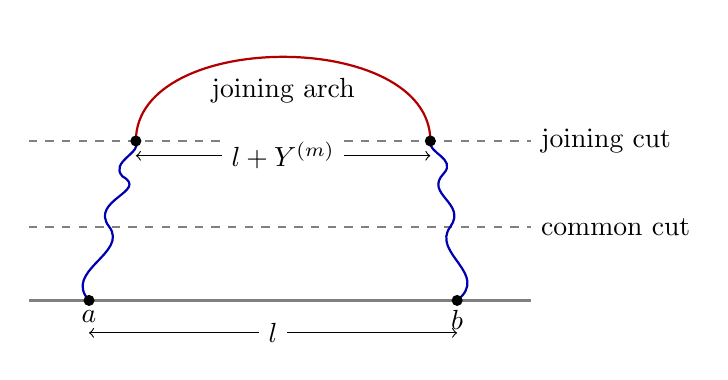
\begin{tikzpicture}[x=0.85cm,y=0.75cm,thick]
\draw[gray] (-0.3,0)--(7.2,0);
\draw[dashed,gray] (-0.3,1.25)--(7.2,1.25);
\draw[dashed,gray] (-0.3,2.7)--(7.2,2.7);
\draw[blue!70!black] (0.6,0) .. controls (0.2,0.5) and (1.2,0.8) .. (0.9,1.25)
 .. controls (0.6,1.7) and (1.5,1.85) .. (1.1,2.1)
 .. controls (0.9,2.35) and (1.4,2.5) .. (1.3,2.7);
\draw[blue!70!black] (6.1,0) .. controls (6.6,0.45) and (5.7,0.8) .. (6,1.25)
 .. controls (6.25,1.65) and (5.6,1.8) .. (5.9,2.15)
 .. controls (6.1,2.4) and (5.65,2.5) .. (5.7,2.7);
\draw[red!70!black] (1.3,2.7) .. controls (1.3,4.6) and (5.7,4.6) .. (5.7,2.7);
\fill (0.6,0) circle(2pt) node[below] {$a$};
\fill (6.1,0) circle(2pt) node[below] {$b$};
\fill (1.3,2.7) circle(2pt);
\fill (5.7,2.7) circle(2pt);
\node[right] at (7.2,1.25) {common cut};
\node[right] at (7.2,2.7) {joining cut};
\node at (3.5,3.55) {joining arch};
\draw[<->,thin] (0.6,-0.55)--(6.1,-0.55) node[midway,fill=white] {$l$};
\draw[<->,thin] (1.3,2.45)--(5.7,2.45) node[midway,fill=white] {$l+Y^{(m)}$};
\end{tikzpicture}
\caption{Two independent prefixes meet a common renewal height and are
joined above it. In the restricted small-prefix construction, the prefixes remain near their respective starting ports.
The first $m$ levels with exactly two crossings recover the sampled pair
blocks. This is a schematic: the lattice paths need not be monotone between
these marked levels.}\label{c:pair-figure}
\end{figure}

\begin{lemma}[Sublinear changes of the gap]\label{c:arch-kernel-regularity}
For positive integers $l,l'$ with $l\to\infty$ and $l'/l\to1$,
\[
 K_{l'}/K_l\longrightarrow1.
\]
\end{lemma}
\begin{proof}
For initial separation \(j\), call prefixes of \(m\) pair-blocks good if \(\sum_{i\le m}D_{*,i}<j/4\), of failure probability \(O(m/\sqrt j)\) by truncation. They are disjoint then, and we may join above the attained common level by any half-plane arch joining the endpoints. This gives
\[
 K_j\ge \mathbb E\,[{\bf1}_{\rm good} K_{j+Y^{(m)}}].
\]
Indeed product probabilities on the pair sequences are ordinary critical weights. The first \(m\) positive base-parallel levels having exactly two crossings of the output are precisely the \(m\) common renewals used: before reaching the joining level each branch must cross each level, and crossing just once is exactly renewal within that branch. The joining level itself has the two prescribed crossings. Thus the construction is injective.



\paragraph{Excluding a jump on a sublinear scale.}
Use monotonicity and the two-sided bounds of order \(l^{-5/4}\). If the conclusion failed, along a sequence there would be drops at least \(\epsilon l^{-5/4}\) between \(l-w\) and \(l+w\) with \(1\le w=o(l)\). For large integer scales \(q\) set \(m=\lfloor\sqrt q\rfloor\); then \(\Pr(Y^{(m)}\le -b q)\ge1/4\) with some small fixed \(b>0\), by Lemma~\ref{c:pair-block-estimates} and symmetry. Also \(\Pr(|Y^{(m)}|>Aq)=O(A^{-1/2})\) by the pair diameter tail and truncation. Fix \(A\) large. Choose \(w\ll q\ll l\) so the variation on \([l+ bq/4,l+(A+b+1)q]\) is \(o(l^{-5/4})\); arbitrarily many disjoint such bands at geometric scales are available between these two scales, and their variations sum to \(O(l^{-5/4})\). At \(j=l+\lfloor bq/2\rfloor\), on good prefixes with \(|Y^{(m)}|\le A q\) the arch factor on the right of the inequality is at least \(K_j-o(l^{-5/4})\). On those also having \(Y^{(m)}\le-bq\), the new gap lies below $l-w$, so the factor gains at least \(\epsilon l^{-5/4}\) over \(K_j\). Good has probability tending to one since $m/\sqrt j=O(\sqrt{q/l})$. The discarded tail loses at most $O(A^{-1/2})K_j$, whereas the gain occurs with probability at least $1/4-O(A^{-1/2})-o(1)$. Taking \(A\) sufficiently large in terms of \(\epsilon\) contradicts the construction inequality.
\end{proof}



\subsection{Concentration under the prescribed-gap law}
\begin{proof}[Proof of Theorem~\ref{c:same-side-law}]
Lemma~\ref{c:arch-kernel-regularity} shows that sublinear perturbations preserve the joining mass.
It remains to transfer the independent-prefix law and bound an unusually
long joining arch. Take \(m=\lfloor l^{1/2-\eta}\rfloor\) for small fixed \(\eta>0\). The good construction exhausts \(1-o(1)\) of total exact arch mass, since \(\sum D_{*,i}/l\to0\) in probability and the joining factor relative to \(K_l\) tends to 1 in probability there (and stays bounded on good prefixes). In the independent pair process the height after \(m\) grows as \(m^{2+o(1)}\) almost surely by the height transform and the power-sum argument of Proposition~\ref{c:renewal}. Each of the two individual cumulative lengths there grows as \((m^2)^{4/3+o(1)}\) by the almost sure individual irreducible-sequence laws, valid also along this subsequence of their renewals. Thus both prefixes' length exponents in \(l\) are arbitrarily close to \(4/3\) with probability tending to one by taking \(\eta\) small, which transfers to good constructed paths by bounded reweighting.



Finally bound the contribution among these paths with joining length above \(\tfrac12 l^{4/3+\epsilon}\). By the atom estimate and translating the first joining endpoint to a fixed origin it is at most
\[
 C m^{-2}\left(C R^{-1/4}+l^{-4/3-\epsilon} R^{13/12+o(1)}\right),\qquad R=l^{1+\gamma}.
\]
Indeed after summing over the other joining endpoint this uses the half-plane diameter bound above \(R\); for smaller diameters the summed length mass with this fixed start is bounded by translating to order \(R\) equivalent starts along the base of a common encompassing convex truncation of size \(O(R)\) and using the free-endpoints length bound \(R^{25/12+o(1)}\) by occupancy. Choose \(\gamma>0\) sufficiently small relative to \(\epsilon\) and then \(\eta>0\) sufficiently small that
\[
 2\eta<\gamma/4,\qquad 2\eta+13\gamma/12<\epsilon.
\]
Both displayed contributions are then $o(l^{-5/4})$. This proves the
half-plane length concentration.

For the hexagon, the prescribed same-side separation satisfies $l\asymp R$.
Proposition~\ref{c:connectors} gives normalizing mass at least
$cl^{-5/4}$ inside the hexagon. The absolute exceptional mass there is
at most the full half-plane exceptional mass, which is $o(l^{-5/4})$.
Dividing by the finite-domain normalizer transfers both length tails.

\end{proof}

\section{Regularity of the strip partition function}\label{c:smoothness-section}

The renewal identity alone gives a tail estimate for the height of one
irreducible bridge.  Prescribing the terminal port requires an estimate
for a single height.  Our first step is to show that the strip partition
function varies smoothly on its natural scale: every fixed forward
difference gains the corresponding power of the strip width.

\begin{proposition}\label{c:strip-smoothness}
Let $B_N$ be the critical mass of strict bridges from one fixed port to
all ports on the opposite pure cut at integral height $N$.  With
$\Delta f_N=f_{N+1}-f_N$, for every fixed integer $\ell\ge0$ and every
$\eta>0$ there is $C_{\ell,\eta}<\infty$ such that
\[
 |\Delta^\ell B_N|\le C_{\ell,\eta}N^{-1/4-\ell+\eta}
 \qquad(N\ge1).
\]
\end{proposition}

The probabilistic application needs precisely Proposition~\ref{c:strip-smoothness}:
its passage to an exact height atom begins in Section~\ref{c:atoms-section}.
We now prove the proposition from the exact finite strip representation and its positive
interpolation spaces.  We state this input before introducing the
holomorphic kernels used to estimate it.  The spectral parameter
$\lambda=\pi/8$ below is unrelated to a path length.
There are three analytic tasks.  We first transport the residual space
to the disk and control its evaluation kernel, including the boundary
column for the non-square-integrable input.  We then recover the residuals at $0$ and $-4$
from their Fourier transforms, retaining every fixed difference in $N$.
Finally a separate positivity argument bounds the denominator away from
zero; only then do we estimate the quotient for $B_N$.

\subsection{The finite strip input}

Put $b=3\lambda$, $C_t(x)=\cosh(t\sqrt x)$,
$\mathcal D(x)=2C_\lambda(x)-1$, and
$a_*=\mathcal D(-4)=2\cos(2\lambda)-1>0$.
Define the positive measure $\mu$ on $(0,\infty)$ by
\begin{equation}\label{c:strip-measure}
 d\mu(x)=\frac{z\mathcal D(z^2)}{\sinh(4\lambda z)}\,dz,
 \qquad x=z^2,\quad z>0.
\end{equation}
For $N\ge1$, set
\[
 \begin{split}
 M_N&=\operatorname{span}\{1,x,\ldots,x^{N-1},
              \partial_t^j C_t|_{t=\lambda}:0\le j<N\},\\
 c_1&=C_{\lambda/2},\quad c_3=C_{3\lambda/2},\quad
 h_0=\mathcal D^{-1},\quad h_1=c_1/\mathcal D,\\
 g&=\int_0^\lambda C_t\,dt,
 \quad F_{0,N}=M_N+\mathbb R c_1,
 \quad G_N=M_N+\mathbb R g.
 \end{split}
\]
Let $\Pi_Nh\in F_{0,N}$ be the unique oblique projection preserving
all pairings against $G_N$ in $L^2(\mu)$, and write
$r_Nh=h-\Pi_Nh$.  The projection is also defined for $c_3$, whose
pairings with $G_N$ are finite although $c_3\notin L^2(\mu)$.

We use the following finite facts from the strip analysis in
\cite[Theorem 2.1 and Lemmas 3.1--3.4]{UniformMarked}.
\begin{enumerate}
\item The above projection exists.  Whenever the denominator is nonzero,
\begin{equation}\label{c:strip-residual-formula}
 B_N=2a_*\left[
 r_Nh_0(-4)-
 \frac{r_N(c_3-h_1)(-4)\,r_Nh_0(0)}{r_N(c_3-h_1)(0)}
 \right].
\end{equation}
The corresponding undivided statement is that there is a scalar $s_N$ such that
$2B_N=4a_*[r_Nh_0(-4)+s_Nr_Nh_0(0)]$ and
$r_N(c_3-h_1)(-4)+s_Nr_N(c_3-h_1)(0)=0$.

\item For $0<t<\lambda$, put $G_{N,t}=M_N+\mathbb R C_t$.
On ordered positive nodes $X=(x_1<\cdots<x_{2N+1})$, the product of
evaluation determinants for $(F_{0,N},G_{N,t})$, times a positive
base weight at every node, defines a positive density whenever its
moments are finite.  Its mean interpolant is the oblique projection
against $G_{N,t}$.  If $e_0c_3$ denotes the interpolation residual at
zero, then $-e_0c_3$ is positive and increasing in each ordered node.
Multiplying the base weight by an increasing positive function increases
its expectation.  Replacing $G_{N,t}$ by $G_N$ is a positive mixture
of these densities.

\item Let $F_N=F_{0,N}+\mathbb R c_3$,
$A_N=\{f\in F_N:f(0)=0\}$, and
$U_N=\{f\in M_N:f(0)=0\}$.  For either determinant-product density
$(F_{0,N},G_{N,t})$ or $(A_N,G_{N,t})$, expectations of
$\prod_i r(x_i)$, with $r(x)=(x+\alpha)/(x+\beta)$ and fixed
$\alpha,\beta>0$, differ by bounded factors from the corresponding
symmetric expectations on $(M_N,M_N)$ or $(U_N,U_N)$.
The factors are uniform in $N,t$ and remain so after any fixed number
of such rational changes of the base weight. This is the interlacing
reduction in the proof of \cite[Lemma 3.2]{UniformMarked}: its positive
weight and exponential-domination hypotheses persist under each such
change, and the bound uses only the range of $\log r$, not $t$.  The two symmetric
expectations themselves differ by a bounded factor.  These statements
follow from interlacing of the positive roots of the compressed
multiplication forms; a codimension-one compression changes the
logarithmic product by at most the range of $\log r$.

\item For the probability measure $\mu_c$ proportional to
$dz/\cosh(cz)$, $x=z^2$, let
$\alpha_c=\pi/(2c)$ and $w_t=\tan^2(\alpha_ct)$.
Then
\begin{equation}\label{c:polynomial-generator}
 A_t(x)=\cos(\alpha_ct)C_t(x),\qquad
 \int A_tA_s\,d\mu_c=\frac1{1-w_tw_s}.
\end{equation}
Thus $A_t=\sum_{j\ge0}P_j(x)w_t^j$ generates orthonormal polynomials
$P_j$ of degree $j$.  The identity and its differentiated forms hold
when $|t|+|s|<c$.
\end{enumerate}
All base weights below have the required exponential domination.  In
particular these inputs apply to $\mu$, to
$dW=z\,dz/\sinh(bz)$, and to $r^jW$ for fixed $j$ and fixed positive
rational function $r$ of the indicated form.  We will prove both the estimates and the nonvanishing
needed to use \eqref{c:strip-residual-formula}.

\subsection{Transforming the residual space}

Set
\[
 v(\omega)=\tan\frac{\pi\omega}{2b},\qquad
 J(\omega)=v'(\omega),\qquad
 Q(v)=\frac{v^2(v^2-v(\lambda)^2)}{1-v^2v(\lambda)^2}.
\]
The strip $|\operatorname{Re}\omega|<b/2$ maps bijectively to the unit
disk.  The rational function $Q$ is an even finite Blaschke product;
its zeros are $0$ with multiplicity two and $\pm v(\lambda)$ with
multiplicity one.  For an even holomorphic function $A$ on the disk,
define
\[
 (T_NA)(\omega)=J(\omega)Q(v(\omega))^N A(v(\omega)).
\]
The factor $Q^N$ encodes exactly the orthogonality conditions against
$M_N$.

Indeed, the cosine transform identifies $h\in M_N^\perp\subset
L^2(\mu)$ with
\begin{equation}\label{c:residual-transform}
 \int h(x)C_\omega(x)\,d\mu(x)=T_NA(\omega).
\end{equation}
The transform is even, has a zero of order $2N$ at zero, and zeros of
order $N$ at $\pm\lambda$.  Dividing by $JQ^N$ therefore gives an
even holomorphic $A$ on the disk.  Conversely these zero conditions
imply the required orthogonality.

Here is the Hilbert-space content of this identification.  Let
$w_\mu(z)$ and $w_W(z)$ be the even extensions of the $z$-densities of
$\mu$ and $W$.  The Fourier datum of the transform $F=T_NA$ is
$f(z)=h(z^2)w_\mu(z)$, so
\[
 F(\omega)=\frac12\int_{\mathbb R}f(z)e^{\omega z}\,dz,
 \qquad
 \|h\|_{L^2(\mu)}^2
 =\frac12\int_{\mathbb R}\frac{|f(z)|^2}{w_\mu(z)}\,dz.
\]
We compare norms while holding $F$, and hence $f$, fixed.  In the
comparison measure $W$, the same transform is represented by
$h_W=h\,d\mu/dW$; its squared norm replaces $w_\mu$ in the last
integral by $w_W$.  Moving to a parallel line multiplies the Fourier
datum by $e^{z\operatorname{Re}\omega}$.  Integrating Plancherel's
identity across the strip supplies the reciprocal weight
$\sinh(bz)/z=1/w_W(z)$.  The conformal Jacobian $J$ then gives the
transported comparison norm
\begin{equation}\label{c:model-norm}
 \mathcal G_N^0(A,A)
 =c_b\int_{|v|<1}|Q(v)|^{2N}|A(v)|^2\,d^2v,
 \qquad c_b>0.
\end{equation}
For completeness, the converse Fourier representation follows by
Fourier transforming the Cauchy--Riemann equation locally in frequency:
the data on parallel lines must have the same exponential multiplier.
Strip square integrability gives the stated weighted $L^2$ data, and
division by the even weight gives $h$.  Thus no unproved surjectivity
of the transform is being used.

Write $\mathcal G_N(A,A)=\|h\|_{L^2(\mu)}^2$ for the norm in
\eqref{c:residual-transform}.  The density ratio of $\mu$ to $W$ is
bounded above and below by positive constants, so
$\mathcal G_N\asymp\mathcal G_N^0$ uniformly in $N$.
More precisely, their difference is a fixed bounded sesquilinear form
on the two traces $T_NA(\pm d_{\mathrm{tr}}+iy)$, for a fixed $d_{\mathrm{tr}}<b/2$ sufficiently
close to $b/2$.  To see this, the difference of the reciprocal Fourier
weights is, up to a fixed factor,
\[
 z^{-1}\left\{\frac{\sinh(4\lambda z)}{\mathcal D(z^2)}
                    -\sinh(bz)\right\}.
\]
It is bounded at zero and is $O(e^{2d_{\mathrm{tr}}|z|})$ at infinity: the terms of
largest exponential order cancel.  Plancherel on the two parallel
lines therefore bounds the difference form by their $L^2$ trace norms.

If $A(v)=\sum_{j\ge0}a_jv^{2j}$, both transported norms are equivalent
to
\begin{equation}\label{c:coefficient-norm}
 \|A\|_N^2=\sum_{j\ge0}\frac{|a_j|^2}{N+j}.
\end{equation}
The boundary phase speed of the finite Blaschke product $Q$ is smooth
and strictly positive.  Hence $|Q(re^{i\theta})|^{2N}$ is bounded
above by $e^{-cN(1-r)}$, and bounded below by
$e^{-CN(1-r)}$ for $r$ near one.  Angular orthogonality of the powers,
followed by radial integration, proves the equivalence.

Every fixed $\ell$th forward difference of $\mathcal G_N^0$ costs
$O_\ell(N^{-\ell})$ as a form in \eqref{c:coefficient-norm}, since
it inserts $(|Q|^2-1)^\ell$ in the area integral.  The same is true
for $\mathcal G_N$.  On each of the fixed interior traces,
$v\to\pm i$ nontangentially at the two ends and $Q(\pm i)=1$; thus
$|1-Q|\le C(1-|Q|)$.  Each difference of $T_N$ inserts $Q-1$,
and comparison with $T_{\lfloor N/2\rfloor}$ costs $O(N^{-1})$.
Interior trace norms are bounded by strip area norms, by the mean-value
inequality for holomorphic functions.  The discrete product rule
therefore gives the same bound for the correction form.  All norms
with finitely shifted indices are equivalent.  Differencing
$\mathcal G_N^{-1}\mathcal G_N=I$ consequently shows that every
$\ell$th difference of the inverse form costs $O_\ell(N^{-\ell})$
as well.

\subsection{The model evaluation kernel}

Denote by $K_N^0(v,u)$ the evaluation kernel for
$\mathcal G_N^0$, analytic in $v$ and anti-analytic in $u$.
Thus, with the inner product linear in its first argument,
$A(u)=\mathcal G_N^0(A,K_N^0(\cdot,u))$ for every even function in the
space and every $|u|<1$. The following bounds are needed also at boundary
points, provided the two variables do not meet on the even diagonal.

\begin{lemma}\label{c:model-kernel}
On every compact subset of the closed bidisk on which
$|1-v^2\overline u^2|>0$, the kernel has continuous boundary values and
\[
 |\Delta^\ell K_N^0(v,u)|\le C_\ell N^{1-\ell},\qquad
 \frac{K_N^0(v,u)}N\longrightarrow
 \frac{O(v)\overline{O(u)}}{1-v^2\overline u^2}.
\]
Here $O$ is even, holomorphic and nonvanishing on a neighborhood of the
closed disk, and positive on both the real and imaginary diameters.
\end{lemma}

\begin{proof}
Let $P_{jk}$ be the Gram matrix of $v^{2j}$ in
\eqref{c:model-norm}, and $R=P^{-1}$.  Thus
$K_N^0(v,u)=\sum_{j,k\ge0}v^{2j}R_{jk}\overline u^{2k}$ in the
open bidisk.  Write $\delta$ for simultaneous forward difference in
$j,k$.  For all fixed nonnegative integers $\ell,s$,
\begin{equation}\label{c:gram-differences}
 |\Delta^\ell\delta^sP_{jk}|
 \le C_{\ell,s}e^{-c|j-k|}(N+j+k)^{-1-\ell-s}.
\end{equation}
In the radial integral the differences insert
$(|Q|^2-1)^\ell(r^4-1)^s$.  For the angular Fourier coefficient,
shift $\theta$ by a sufficiently small fixed imaginary amount in the
direction giving decay in $|j-k|$.  The continued expression
$Q(re^{i\theta})Q(re^{-i\theta})$ equals one at $r=1$.
Its positive radial logarithmic derivative stays positive under this
small shift, and compactness away from the boundary gives a strict
bound below one there.  It therefore decays as $e^{-c(1-r)}$ and
differs from one by $O(1-r)$.  Radial integration proves
\eqref{c:gram-differences}.

The inverse matrix satisfies
\begin{equation}\label{c:inverse-gram-differences}
 |\Delta^\ell\delta^sR_{jk}|
 \le C_{\ell,s}e^{-c|j-k|}(N+j+k)N^{-\ell}
                   (1+\min\{j,k\})^{-s}.
\end{equation}
First take $\ell=s=0$.  We use the exponential-conjugation argument
for localized inverses; compare Jaffard~\cite[Proposition 2]{Jaffard1990}.
The parameter differences will be retained explicitly below.
Conjugating $P$ by diagonal factors
$\sqrt{N+j}$ gives a positive operator with bounded positive inverse,
by \eqref{c:coefficient-norm}.  Conjugation of this normalized operator
by weights of sufficiently small exponential logarithmic slope changes
it by an arbitrarily small operator norm, by row and column sums in
\eqref{c:gram-differences}.  Its inverse remains bounded.  Truncate
these weights and pass to the limit to obtain exponential decay of
inverse entries, proving the undifferenced case.

Here are details for the differences.  Write
$(SA)_{jk}=A_{j+1,k+1}$, so $\delta A=SA-A$.  The half-line matrix
product has the exact shift rule
\[
 S(AB)=(SA)(SB)+E(A,B),\qquad
 E(A,B)_{jk}=A_{j+1,0}B_{0,k+1}.
\]
In particular $PR=I$ gives, with the $N$ dependence explicit in the
second identity,
\[
 \delta R=-R(\delta P)SR-R E(P,R),
 \qquad
 \Delta R_N=-R_N(\Delta P_N)R_{N+1}.
\]
The first identity displays the boundary contribution that is absent
from a difference in $N$.  Bounds of the form in
\eqref{c:inverse-gram-differences}, with $(N+j+k)^a$ in place of its
first power, compose under matrix multiplication by adding the orders
$a$; convolution of exponential decays absorbs every fixed polynomial
in index distance.  The boundary term $E(P,R)$ and its fixed index
shifts have exponential decay in $j+k$, which pays every displayed
index-decay factor.  First establish all pure $N$ differences from the
second identity.  Then induct on $s$ in the first identity, treating
every fixed $\ell$ at each step.  Discrete product rules use only
lower-order index differences of $R$; the extra difference on $P$ and
the boundary localization give the additional index decay.  Together
with \eqref{c:gram-differences}, these bounds prove
\eqref{c:inverse-gram-differences}.

These estimates also give convergence at the boundary off the even
diagonal.  On each matrix diagonal $j-k$ fixed, put
$n=\min\{j,k\}$ and use a smooth dyadic partition in $n$.
The variable factor is $(v^2\overline u^2)^n$.
Summing by parts $s$ times, and then summing the exponentially decaying
matrix diagonals, bounds the block $n\asymp m$ of
$N^{\ell-1}\Delta^\ell K_N^0$ by $C_sm^{2-s}$, uniformly whenever
$|1-v^2\overline u^2|$ is bounded below.  Choosing $s>2$ gives
uniform convergence of these dyadic blocks and the asserted difference
bound and continuity.  In the open bidisk this sum agrees with the
absolutely convergent kernel, so it gives its boundary values.

For fixed $j,k$, boundary radial Laplace integration shows that
$NP_{jk}$ tends to a positive Toeplitz matrix.  Its symbol is a
positive constant times the reciprocal boundary phase speed of $Q$,
restricted to even powers.  Exponential matrix decay allows passage
to the limit in both inverse identities, so $R_{jk}/N$ tends to the
inverse of this Toeplitz form.  Factor the positive symbol as
$1/|O|^2$, by harmonically extending its logarithm and taking a
harmonic conjugate, normalized by $O(0)>0$.  This is the usual outer
factor construction; see Simon~\cite[Section 5]{Simon2005Szego}.
Real analyticity,
evenness, and reflection symmetry of the symbol give the asserted
analytic continuation, nonvanishing, and symmetries of $O$.
In particular $O$ is real and cannot change sign on either diameter.
Multiplication by $1/O$ is an isometry from the resulting weighted
even Hardy space onto the ordinary even Hardy space.  The latter has
kernel $(1-v^2\overline u^2)^{-1}$.  This identifies the limit;
the same summable dyadic tail bound makes the convergence uniform on
the stated compact sets.
\end{proof}

The model has now isolated the only large part of the evaluation
kernel.  The remaining change of measure contributes a bounded vector,
which is small enough for every residual estimate below.

Let $K_N$ denote the kernel for $\mathcal G_N$.  If
$u=v(t)$, $0\le t\le\lambda$, or $t\uparrow b/2$, then
\begin{equation}\label{c:kernel-correction}
 \|\Delta^\ell(K_N(\cdot,u)-K_N^0(\cdot,u))\|_N
 \le C_\ell N^{-\ell}.
\end{equation}
At $t=b/2$, where $u=1$, the difference of columns has a limit in
$\|\cdot\|_N$.  Neither full boundary column is asserted to be a
finite-norm vector.  We define $K_N(\cdot,1)$ as the model boundary
column plus this finite-norm correction, with evaluations in the open
disk obtained as limits from inside.
Indeed the pairs formed by a point on either fixed interior trace and
these $u$ are uniformly off the even diagonal.  On the traces,
\[
 |J|\asymp e^{-\pi|y|/b},\qquad
 1-|Q|\gtrsim e^{-\pi|y|/b}.
\]
Lemma~\ref{c:model-kernel} and discrete product rules therefore give
\[
 \|\Delta^\ell(T_NK_N^0(\cdot,u))\|_{L^2(\{\pm d_{\mathrm{tr}}+iy\})}
 \le C_\ell N^{-\ell}.
\]
For example the undifferenced integrand is bounded by
\[
 CN e^{-\pi|y|/b}\exp\{-cNe^{-\pi|y|/b}\}.
\]
Its squared integral is bounded; each difference supplies its stated additional
factor.  Apply the bounded correction form to this column and solve
with $\mathcal G_N^{-1}$.  The resolvent identity and the inverse
difference bounds prove \eqref{c:kernel-correction}.  Dominated
convergence on the traces gives its endpoint interpretation.

Evaluation at a fixed interior disk point costs $O(\sqrt N)$ in
\eqref{c:coefficient-norm}.  Consequently, for $v,u$ corresponding to
$0\le t\le\lambda$, the actual kernel has the same strictly positive
leading limit after division by $N$, with $\ell$th differences
$O(N^{1-\ell})$.  The same holds when exactly one variable is $1$.

\subsection{Residual estimates at the two evaluation points}

We prove the following bounds, which are the full analytic input to the
quotient in \eqref{c:strip-residual-formula}:
\begin{equation}\label{c:residual-estimates}
 \begin{split}
 |\Delta^\ell r_Nh_j(-a)|
     &\le N^{-1+b\sqrt a/\pi-\ell+o(1)}\quad(j=0,1),\\
 |\Delta^\ell r_Nc_3(-a)|
     &\le N^{b\sqrt a/\pi-\ell+o(1)}\quad(a=0,4),\\
 -r_Nc_3(0)&\ge c>0.
 \end{split}
\end{equation}
All orders $\ell$ are fixed.  The estimates with $o(1)$ mean that
each fixed positive exponent slack is allowed, with its own constant.

First take the orthogonal residual against $M_N$ alone.  For input
$h=h_j$ its transform is $T_NA_{h,N}$, where $A_{h,N}$ represents the
functional obtained by pairing $h$ with the residual space.  Write
\[
 h(z^2)=\int_{\mathbb R}f_h(y)\cos(yz)\,dy.
\]
The function $f_h$ is integrable against $e^{u|y|}$ for each
$u<\pi/(3\lambda)=\pi/b$.  This follows by Fourier inversion and
shifting within closed narrower strips: the first zeros of
$\mathcal D(z^2)$ have imaginary part $\pi/(3\lambda)$, and the
functions decay exponentially along every such horizontal line.
Thus the functional on $A$ is
$\int f_h(y)(T_NA)(iy)\,dy$.

On $\|A\|_N\le1$, the area mean-value bound and comparison to
$T_{\lfloor N/2\rfloor}$ give
\[
 |(\Delta^\ell T_NA)(iy)|
 \le C_\ell N^{-\ell}
       \exp\{-cNe^{-\pi|y|/b}\}.
\]
Indeed $1-|Q(v(iy))|\gtrsim e^{-\pi|y|/b}$ and
$|1-Q|\lesssim1-|Q|$ there.  Integrating against $f_h$, then using
the inverse-form differences, yields
\begin{equation}\label{c:h-vector-bound}
 \|\Delta^\ell A_{h,N}\|_N\le N^{-1-\ell+o(1)}.
\end{equation}
For an input $C_s$ with $0\le s<b/2$, the representing vector is
instead $J(s)Q(v(s))^NK_N(\cdot,v(s))$.  As $s\uparrow b/2$, all
finite projection pairings and the residual transforms on compact
subsets of the strip converge.  Thus the formula extends to $c_3$
using the boundary column just constructed and $Q(1)=1$; it does not
assert a bounded Hilbert-space evaluation functional at $u=1$.

We now impose the one remaining oblique constraint.  Put
$u_0=v(\lambda/2)$.  The transform of $r_Nh$ is $T_N$ applied to
\begin{equation}\label{c:oblique-vector}
 A_{h,N}-K_N(\cdot,u_0)
       \frac{\chi_N(A_{h,N})}{\chi_N(K_N(\cdot,u_0))},
\end{equation}
where $\chi_N$ averages values at $v(t)$, $0\le t\le\lambda$,
with probability proportional to $J(t)|Q(v(t))|^Ndt$.
To check the formula, orthogonality to $M_N$ is already encoded in
$T_N$, and $\int_0^\lambda C_tdt=g$.  On this interval $Q$ has
constant sign away from its zeros, so this last condition is precisely
$\chi_N=0$.

Every fixed $\ell$th difference of the probabilities defining
$\chi_N$ is $O_\ell(N^{-\ell})$ in total variation.  Divide their
exponential base by its maximum.  Differencing inserts powers of the
gap to one.  Integrals at exponents $N/2$ and $N$ are comparable:
the gap vanishes to finite order at its finitely many maxima, by
analyticity, and the one-dimensional radial Laplace estimate applies
in disjoint neighborhoods of them.  Normalization and the quotient
difference rule give the claim.  Kernel positivity and its leading
limit now show
\[
 \chi_N(K_N(\cdot,u_0))\ge cN,
 \qquad
 |\Delta^\ell\chi_N(K_N(\cdot,u_0))|
 \le C_\ell N^{1-\ell}.
\]
For $h_j$, the subtracted vector in \eqref{c:oblique-vector} has the
same bound as \eqref{c:h-vector-bound}: use the $O(\sqrt N)$ interior
evaluation bound, the $O(\sqrt N)$ column norm, and the denominator
of order $N$, with their corresponding difference bounds.  For $c_3$,
the scalar multiplier of the interior column has $\ell$th differences
$O_\ell(N^{-\ell})$.  The model columns at $1$ and $u_0$ have
$T_N$-images on the imaginary axis bounded by $O(N^{-\ell})$
after $\ell$ differences, by the off-diagonal kernel estimate; their
finite-norm corrections satisfy the same bound.  We have proved,
with $F_{h,N}(\omega)=\int(r_Nh)C_\omega\,d\mu$, that
\begin{equation}\label{c:transform-uniform}
 |\Delta^\ell F_{h,N}(iy)|\le N^{a_h-\ell+o(1)},\qquad
 a_{h_0}=a_{h_1}=-1,\quad a_{c_3}=0,
\end{equation}
uniformly for $y\in\mathbb R$.

\paragraph{Growth on a shifted contour.}
The bound at $-4$ requires a contour argument; it is not an evaluation
on the integration axis.  For $h=h_0,h_1,c_3$, put
\[
 \rho_{h,N}(z)
 =(r_Nh)(z^2)\frac{z\mathcal D(z^2)}{\sinh(4\lambda z)}.
\]
We first prove that, for every fixed $Y>0$ which is not an even integer,
\begin{equation}\label{c:contour-growth}
 \int_{\mathbb R}|\rho_{h,N}(z+iY)|\,dz
 \le C_Y N^{bY/\pi+C},
\end{equation}
where the additive exponent $C$ is independent of $Y$.  This uniformity
will allow us to choose $Y$ after fixing the desired difference order.
The factors $\mathcal D$ remove the poles of $h_0,h_1$ in this product.

In the orthogonal polynomial expansion
\eqref{c:polynomial-generator} with $c=b$,
coefficients of an element of $F_{0,N}$ beyond index $N-1$ have the
form
\[
 q^jp(j)+d_0q_1^j,\qquad \deg p<N,
 \quad 0<q_1=w_{\lambda/2}<q=w_\lambda<1.
\]
Divide by $q^j$ and take $N$ consecutive forward differences to bound
$d_0$ by $e^{O(N)}$ on the unit sphere.  Lagrange interpolation on
$N$ consecutive indices bounds the remaining polynomial.  Consequently
the coefficients decay exponentially beyond $C'N$, relative to the
norm, for a fixed sufficiently large $C'$.
Fix $2\lambda<c<b$ and repeat the coefficient-tail argument in the
orthonormal polynomial basis for $\mu_c$. For each $f\in F_{0,N}$,
its truncation at degree $O(N)$ approximates $f$ with exponentially
small relative $\mu_c$-norm error. The small-circle generating-function
bound gives $|P_j^{(c)}(z^2)|\le C_c^{j+1}e^{cz/4}$ for this basis.
Choosing a fixed $C'$ sufficiently large therefore makes the
truncation's $\mu_c$-norm on $z>C'N$ exponentially small relative to
$\|f\|_{\mu_c}$. By the triangle inequality, a fixed positive fraction
of the full $\mu_c$-norm of $f$ lies on $z\le C'N$. On this interval
the density ratio $d\mu_c/d\mu_b$ is at most $e^{O(N)}$, and hence
\[
 \|f\|_{\mu_c}\le e^{O(N)}\|f\|_{\mu_b},\qquad f\in F_{0,N}.
\]
All constants here may depend on the fixed $c$, not on $N$.

Pairing against $c_3$ with $\mu$ has norm at most a fixed power of
$N$ on this space.  On $z\le N^2$ use Cauchy--Schwarz; since
$c_3(z^2)^2d\mu/dz=O(1+z)$, its truncated squared integral is
polynomial in $N$.  Beyond $N^2$ use the just established $\mu_c$
comparison: the other factor in Cauchy--Schwarz decays as
$e^{-(b-c)z}$, which dominates $e^{O(N)}$.  Thus the orthogonal
projection of $c_3$ on $M_N$ has polynomially bounded norm.  Its
extra oblique projection term also does, by
\eqref{c:oblique-vector}; for $h_j$ this already follows from
\eqref{c:h-vector-bound}.

Finally the generating formula on
$|w_t|=\exp(-1/(j+1))$ gives
\[
 |P_j((z+iY)^2)|
 \le C_Y(j+1)^{1/2+bY/\pi}e^{b|z|/2}.
\]
Here the corresponding parameter satisfies
$|\operatorname{Re}t|<b/2$ and
$|\operatorname{Im}t|\le(b/\pi)\log(j+1)+O(1)$.
Summing with the coefficient bounds, and including the elementary
direct inputs, proves \eqref{c:contour-growth}: multiplication by the
density leaves integrable exponential decay in $|z|$.  In particular
the exponent has coefficient $bY/\pi$ and an additive constant
independent of $Y$, as required.

\paragraph{Recovering the two evaluations.}
Fix the difference order $\ell$ and an arbitrarily small $\eta>0$, and
put $S_N=(b/\pi+\eta)\log N$.  In the full even Fourier integral for
$F_{h,N}(iy)$, shift the $z$ contour to $\operatorname{Im}z=Y$.
The only crossed poles are the simple poles of $1/\sinh(4\lambda z)$
at $z=2in$, $n\ge1$.  The growth bound gives, for $y\ge S_N$,
\begin{equation}\label{c:contour-expansion}
 F_{h,N}(iy)=\sum_{0<2n<Y}b_{n,N}e^{-2ny}
                  +O_Y(e^{-Yy}N^{bY/\pi+C}),
\end{equation}
where $b_{1,N}$ is a fixed nonzero multiple of $r_Nh(-4)$.
Apply \eqref{c:contour-expansion} also at $N+1,\ldots,N+\ell$,
keeping the same $S_N$, and take differences.  At
$y=S_N+j$ for enough consecutive integers $j\ge0$, the exponentials
form a fixed Vandermonde system.  Choose the non-even height $Y>2$
sufficiently large depending on $\ell,\eta$, and then let $N$ tend to
infinity.  Since $C$ is independent of $Y$, the remainder
$N^{-\eta Y+C}$ is negligible at the required difference order.
Equation~\eqref{c:transform-uniform} then bounds every coefficient
$e^{-2nS_N}\Delta^\ell b_{n,N}$ by
$N^{a_h-\ell+o(1)}$.  For $n=1$ this gives
\[
 |\Delta^\ell r_Nh(-4)|
 \le N^{a_h+2b/\pi+2\eta-\ell+o(1)}.
\]
Letting $\eta$ be arbitrarily small proves the claimed exponent.
The same expansion bounds the integral over $y\ge S_N$ by
$N^{a_h-\ell+o(1)}$.  Below $S_N$, integrate
\eqref{c:transform-uniform}; its logarithmic factor is absorbed in
$o(1)$.  Fourier inversion at $z=0$, where the density of $\mu$ is
positive and finite, gives the first two lines of
\eqref{c:residual-estimates} also at $a=0$.

\subsection{A uniform nonzero denominator}

It remains to prove $-r_Nc_3(0)\ge c$.  An upper estimate for the
residual would not suffice to divide by it.
First replace $G_N$ by $G_{N,t}$, $0<t<\lambda$, and use the
comparison measure $W$ in both projection and transform.  Its kernels
are exactly $K_N^0$, and $\chi_N$ becomes point evaluation at $v(t)$.
Apart from the fixed positive factor $J(b/2)$, the residual transform is
$J(iy)Q(v(iy))^N$ times
\[
 K_N^0(v,1)-K_N^0(v,u_0)
          \frac{K_N^0(v(t),1)}{K_N^0(v(t),u_0)},
 \qquad v=v(iy).
\]
After division by $N$, Lemma~\ref{c:model-kernel} gives a limit
uniform on the imaginary diameter.  At $v=\pm i$, its sign is the
sign of
\[
 \frac12-
 \frac{1-v(t)^2u_0^2}{(1+u_0^2)(1-v(t)^2)},
\]
which is strictly negative, uniformly for $0\le t\le\lambda$.
Indeed the second term is at least $1/(1+u_0^2)>1/2$.
The remaining factors $O$ are positive on both diameters, with uniform
positive bounds on the compact sets in question.

Fourier inversion at zero integrates the bracket divided by $N$ against
\[
 cNJ(iy)Q(v(iy))^Ndy,\qquad c>0.
\]
This positive measure has mass bounded above and below and concentrates
at $y\to\pm\infty$: on the imaginary diameter $Q\ge0$,
$1-Q\asymp e^{-\pi|y|/b}$, and
$J\asymp e^{-\pi|y|/b}$.
The boundedness supplied by Lemma~\ref{c:model-kernel} and the negative
endpoint limit therefore give the desired lower bound for $W$,
uniformly in $t$.

To pass to $\mu$, its exact density ratio to $W$ is
\[
 \frac{d\mu}{dW}
 =\frac{(2u-1)^2(2u+1)}{4u(2u^2-1)},
 \qquad u=\cosh(\lambda\sqrt x).
\]
It is positive and smooth on $[0,\infty)$ and eventually increasing.
For $r(x)=(x+2)/(x+1)$, choose a fixed integer $j>0$ so that
$\mu/(r^jW)$ is increasing: on a compact interval the negative part
of the logarithmic derivative is bounded, while
$-(\log r)'$ is strictly positive; outside it the original derivative
is already nonnegative.  The ordered association input then bounds
the expectation of $-e_0c_3$ for $\mu$ below by that for $r^jW$.

Each multiplication of the base weight by $r$ changes this expectation
by only a bounded factor.  Indeed it multiplies it by the ratio of the
characteristic-product expectations of $\prod_i r(x_i)$ under
$(A_N,G_{N,t})$ and $(F_{0,N},G_{N,t})$ at the current base weight.
The interlacing input compares the first to $(U_N,U_N)$ and the second
to $(M_N,M_N)$; symmetric codimension-one compression compares these
last two.  The bounded range of $\log r$ gives a uniform constant at
each step, independent of $N,t$.  After the fixed number $j$ of steps,
the lower bound therefore remains positive.  Finally integrate the
positive $G_{N,t}$ mixture to obtain it for $G_N$.
This proves the last line of \eqref{c:residual-estimates}.

\paragraph{The quotient.}
We can now finish Proposition~\ref{c:strip-smoothness}.
The denominator $r_N(c_3-h_1)(0)$ in
\eqref{c:strip-residual-formula} is bounded away from zero for all
sufficiently large $N$, because
$-r_Nc_3(0)\ge c$ and $|r_Nh_1(0)|\le N^{-1+o(1)}$.
Its reciprocal has $\ell$th differences $N^{-\ell+o(1)}$, by the
discrete inverse rule and \eqref{c:residual-estimates}.  In the
numerator, $r_Nh_0(-4)$ has differences
$N^{-1+2b/\pi-\ell+o(1)}$, while the product of
$r_N(c_3-h_1)(-4)$ and $r_Nh_0(0)$ has exactly the same bound.
Apply the discrete product and quotient rules.  Since
$2b/\pi=3/4$, the resulting exponent is $-1/4-\ell+o(1)$,
as asserted.  For each fixed $\ell$ and exponent slack, the finitely
many remaining values of $N$ are absorbed in $C_{\ell,\eta}$.

\section{Exact height and displacement atoms}\label{c:atoms-section}

We now turn strip regularity into estimates for a bridge with a prescribed
terminal port.  Throughout this section, $p$ is the probability law of one
irreducible bridge from a fixed port.  Write $H$, $Z$, $L$, and $D$
for its positive integral height, transverse displacement, number of visited
triangle centers, and diameter.  The vector $X=(H,Z)$ takes values on the
actual row-staggered lattice; an atom outside this lattice is zero.  For
independent copies, put
\[
 S_k=X_1+\cdots+X_k,\qquad
 T_k=L_1+\cdots+L_k.
\]
Independence is used between whole pieces, never between coordinates of
one piece.

We use the renewal identity and one-piece estimates stated earlier:
\begin{equation}\label{c:renewal-atom-inputs}
 \sum_{h\ge0}B_hz^h=\frac1{1-\mathbb E_p z^H},\qquad
 B_0=1,\quad B_h\asymp(1+h)^{-1/4},
\end{equation}
and, for $x,t\ge1$ and $u\downarrow0$,
\begin{equation}\label{c:tail-atom-inputs}
 \begin{split}
 p(H>x)+p(D>x)&\le Cx^{-3/4},\\
 p(L>t)&\le t^{-9/16+o(1)},\qquad
 1-\mathbb E_p e^{-uL}=u^{9/16+o(1)}.
 \end{split}
\end{equation}
The first identity implies
$1-\mathbb E_p e^{-sH}\asymp s^{3/4}$.
These are statements under $p$, before conditioning on an endpoint.

\subsection{An atom of the one-piece height}

The extra information supplied by strip regularity is one full power of
height decay beyond the tail bound.  This is the estimate that rules out
bridges made from too few irreducibles at one prescribed endpoint.

\begin{proposition}\label{c:height-atom}
For every $\eta>0$ there is $C_\eta<\infty$ such that
\[
 p(H=n)\le C_\eta n^{-7/4+\eta}\qquad(n\ge1).
\]
\end{proposition}

\begin{proof}
Let $b(z)=\sum_{m\ge0}B_mz^m$.  Fix $n\ge2$, set
$r=e^{-1/n}$, and write $s=\min\{1,n^{-1}+|\theta|\}$ for
$-\pi\le\theta\le\pi$.  The height tail gives
\[
 |1-\mathbb E_p(re^{i\theta})^H|
 \le C\mathbb E_p\min\{1,sH\}\le Cs^{3/4}.
\]
Thus $|b(re^{i\theta})|\ge cs^{-3/4}$.  In particular $b$ has no
zero on this circle, as also follows from its renewal representation.

For every fixed integer $k\ge0$ and every $\delta>0$, the strip
differences of Proposition~\ref{c:strip-smoothness} imply
\begin{equation}\label{c:b-angular-derivatives}
 \left|\partial_\theta^k b(re^{i\theta})\right|
 \le C_{k,\delta}s^{-3/4-k-\delta}.
\end{equation}
Here are the details of the summation estimate.  Choose a smooth dyadic
partition of unity on the positive integers.  On $m\asymp M$, discrete
product rules and the strip differences bound every $j$th difference of
$m^kB_mr^m$ times the cutoff by
$C_{j,k,\delta}M^{k-1/4-j+\delta}e^{-M/(Cn)}$.
Summation by parts $j$ times, together with the trivial sum bound, gives
\[
 C_{j,k,\delta}M^{3/4+k+\delta}
 e^{-M/(Cn)}(1+M|\theta|)^{-j}.
\]
Choose $j>3/4+k+\delta$ and sum over dyadic $M$.  The terms with
$M\le s^{-1}$ form a geometric sum; the remaining terms are bounded by
the oscillatory factor or the exponential cutoff.  This proves
\eqref{c:b-angular-derivatives}.

Differentiating the reciprocal twice now gives
\[
 \left|\partial_\theta^2 b(re^{i\theta})^{-1}\right|
 \le C_\delta s^{-5/4-2\delta}.
\]
Consequently its integral over $[-\pi,\pi]$ is at most
$C_\delta n^{1/4+2\delta}$.  Since
$\mathbb E_pz^H=1-b(z)^{-1}$, the $n$th Fourier coefficient on this
circle, integrated by parts twice, satisfies
\[
 r^n p(H=n)
 \le\frac1{2\pi n^2}
 \int_{-\pi}^{\pi}\left|
 \partial_\theta^2 b(re^{i\theta})^{-1}\right|\,d\theta
 \le C_\delta n^{-7/4+2\delta}.
\]
The boundary terms vanish by periodicity, $r^n=e^{-1}$, and $\delta$
is arbitrary.
\end{proof}

\subsection{Two forms of displacement smoothing}

We need both a planar atom bound and a bound summed over possible heights.
The latter is stronger than merely summing the planar bound over all
heights, since the height distribution has an infinite tail.

\begin{proposition}\label{c:planar-atoms}
There is $C<\infty$ such that, for every integer $k\ge1$,
\begin{equation}\label{c:two-atom-bounds}
 \sup_w\Pr(S_k=w)\le Ck^{-8/3},\qquad
 \sum_{m\in\mathbb Z}\sup_{H(w)=m}\Pr(S_k=w)
 \le Ck^{-4/3}.
\end{equation}
\end{proposition}

\begin{proof}
We first establish a directional window for one piece.  There are constants
$0<c_0<C_0<\infty$ and $c_1>0$ such that, uniformly over unit vectors $e$
and all sufficiently large $x$,
\begin{equation}\label{c:directional-window}
 p\{c_0x\le |e\cdot X|\le C_0x\}\ge c_1x^{-3/4}.
\end{equation}
Use bridges of heights in $[x,2x]$ and terminal ports in a transverse
interval of length comparable to $x$.  The point-to-point connector lower
bound is $cx^{-5/4}$ at each such port.  The two intervals of bounded
positive and negative slope may be chosen so that their displacements
have projection at least a fixed multiple of $x$ in any prescribed
direction.  Compactness of the unit circle makes the constants uniform.
Summing over heights and ports gives critical mass at least $cx^{3/4}$.

By the renewal factorization, this is a sum of probabilities for $S_k$.
The terms $k>Ax^{3/4}$ have total mass at most
\[
 \sum_{k>Ax^{3/4}}e^2
   (\mathbb E_p e^{-H/x})^k
 \le Cx^{3/4}e^{-cA}.
\]
Fix $A$ large.  Some $k\le Ax^{3/4}$ therefore has probability bounded
below of producing an absolute projection comparable to $x$.
The probability of an increment with $D>C_0x$ is at most
$CA C_0^{-3/4}$, while
\[
 \mathbb E\sum_{i\le k}|e\cdot X_i|
       \mathbf1_{\{|e\cdot X_i|<c_0x\}}
 \le CA c_0^{1/4}x.
\]
The second estimate follows by integrating the diameter tail; fixed
lattice conversion constants are absorbed in $C$.  Choose $C_0$ large
and $c_0$ small.  With a fixed positive probability an increment then
lies in the window in \eqref{c:directional-window}.  A union bound and
$k\le Ax^{3/4}$ prove that display.

Let $\varphi(\theta)=\mathbb E e^{i\theta\cdot X}$, using any fixed
integer coordinates for the displacement lattice.  An independent copy
$X'$ lies in a fixed bounded set with probability bounded below.  Apply
\eqref{c:directional-window} in direction $\theta/|\theta|$, with
$x$ a sufficiently small fixed multiple of $|\theta|^{-1}$.  On the
resulting event, $|\theta\cdot(X-X')|$ stays between two positive
constants less than $\pi$.  Hence
\[
 1-|\varphi(\theta)|^2
 =\mathbb E[1-\cos(\theta\cdot(X-X'))]
 \ge c|\theta|^{3/4}
\]
near zero.  The directional windows also show that the affine span of the
support is two-dimensional.  Its difference group is therefore a
full-rank lattice subgroup.  There are only finitely many points of the
lattice torus where $|\varphi|=1$; near each, its modulus is a translate
of the modulus near zero.  On the remaining compact set it is strictly
less than one.  Fourier inversion gives
\[
 \sup_w\Pr(S_k=w)
 \le C\int_0^1 e^{-ckr^{3/4}}r\,dr+Ce^{-ck}
 \le Ck^{-8/3}.
\]
This also explains why no aperiodicity assumption beyond the actual
support lattice is needed.

It remains to sum the heightwise supremums.  For a nonnegative measure
$q$ on the displacement lattice, set
\[
 \|q\|_{1,\infty}
 =\sum_m\sup_{H(w)=m}q(w).
\]
Convolution satisfies
$\|q*r\|_{1,\infty}\le\|q\|_{1,\infty}\|r\|_1$.
The first bound of \eqref{c:two-atom-bounds} immediately bounds the sum
over $m\le2k^{4/3}$ by $Ck^{-4/3}$.

For a dyadic shell $m\asymp\Lambda k^{4/3}$, $\Lambda\ge2$, split the $k$ pieces
into sixteen independent blocks with sizes comparable to $k$; bounded
$k$ can be absorbed into the constant.  Each block has planar atoms at
most $Ck^{-8/3}$.  Also a block height exceeds $t\ge k^{4/3}$ with
probability at most $Ckt^{-3/4}$: split at increments larger than $t$
and use the truncated first moment for the rest.

Suppose first that one block has height at most $k^{4/3}\sqrt\Lambda$.
For large $\Lambda$, another has height at least $c\Lambda k^{4/3}$.  The first
restricted block has $\|\cdot\|_{1,\infty}$ at most
$C\sqrt\Lambda\,k^{-4/3}$ by its planar atom bound, while the latter event
has probability at most $C\Lambda^{-3/4}$.  Convolve with the remaining blocks
and sum over the finitely many choices.  This gives
$C\Lambda^{-1/4}k^{-4/3}$ for the shell.  If all sixteen block heights exceed
$k^{4/3}\sqrt\Lambda$, impose the planar atom on one block and the probability
bound $C\Lambda^{-3/8}$ on each of the other fifteen.  There are
$O(\Lambda k^{4/3})$ heights in the shell, so this case costs at most
$C\Lambda^{-37/8}k^{-4/3}$.  Both bounds are summable over dyadic $\Lambda$.
Increasing the constant handles the finitely many small $\Lambda$ and bounded
$k$, completing the proof.
\end{proof}

\section{Prescribed ports on parallel sides}\label{c:parallel-section}

The strip estimates above concern a fixed initial port and all terminal
ports.  We now prescribe the second port as well.  The connector
construction gives the required normalization: when the height is $h$
and the transverse displacement is $O(h)$, the critical mass between the
two ports is at least $ch^{-5/4}$.  The constant is uniform over fixed
compact nondegenerate scaled geometries.  The same construction lies in
a convex pure-sided domain if both ports have clearance comparable to
$h$ from every side other than the opposite parallel sides containing
them.  We will show that the exceptional mass in the entire strip is
$o(h^{-5/4})$.

\begin{theorem}\label{c:parallel}
Fix a bound on the ratio of transverse displacement to height.  For
compatible prescribed ports on two parallel pure cuts at integral height
$h\to\infty$, normalize the critical bridge weights by their total
mass.  For every $\epsilon>0$,
\[
 \Pr\{h^{4/3-\epsilon}\le L
                       \le h^{4/3+\epsilon}\}\longrightarrow1.
\]
The convergence is uniform under the fixed displacement bound.  It also
holds in convex pure-sided domains in a fixed compact family of
nondegenerate scaled geometries, with the ports on opposite parallel
sides and with order-$h$ clearance from every other side.
\end{theorem}

\begin{proof}
It is enough to treat $0<\epsilon<1$.  Let $w$ be the prescribed
displacement, with $H(w)=h$.  Unique
factorization writes its bridge mass as
$\sum_{k\ge1}\Pr(S_k=w)$.  We first discard very small and very large
numbers of pieces without imposing a length restriction.

Fix a small $\xi>0$.  Put $K=h^{3/4-\xi}$ and
$a=h^{1-\tau}$, where $0<\tau<8\xi/21$.  For $k\le K$, the event
$\sum_{i\le k}H_i=h$ with every $H_i<a$ has probability at most
\[
 e^{-h/a}\bigl(\mathbb E[e^{H/a};H<a]\bigr)^k
 \le\exp\{-h^\tau+Cka^{-3/4}\}.
\]
We used $e^t-1\le et$ for $0\le t\le1$ and
$\mathbb E[H;H<a]\le Ca^{1/4}$.  Since
$ka^{-3/4}\le h^{-\xi+3\tau/4}$, summing these probabilities over
$k\le K$ is smaller than every inverse power of $h$.

If some $H_i\ge a$, fix its index and condition on the other pieces.
Proposition~\ref{c:height-atom}, followed by the heightwise bound of
Proposition~\ref{c:planar-atoms}, gives
\begin{align*}
 &\Pr\{S_k=w,\ H_i\ge a\}\\
 &\quad\le
 \sup_{n\ge a}p(H=n)
 \sum_m\sup_{H(v)=m}\Pr(S_{k-1}=v)
 \le a^{-7/4+o(1)}C(1+k)^{-4/3}.
\end{align*}
For $k=1$ the remaining sum is interpreted as the unit mass at zero.
Summing over the candidate index and then over $k\le K$ gives
\[
 C a^{-7/4+o(1)}K^{2/3}
 =h^{-5/4-2\xi/3+7\tau/4+o(1)}
 =o(h^{-5/4}).
\]
This is the step that needs both the one-piece height atom and the
heightwise supremum estimate.

For $k>h^{3/4+\xi}$, height discount alone gives
\[
 \sum_{k>h^{3/4+\xi}}\Pr\Bigl\{\sum_{i\le k}H_i=h\Bigr\}
 \le e\sum_{k>h^{3/4+\xi}}(\mathbb E e^{-H/h})^k
 \le Ch^{3/4}e^{-ch^\xi}.
\]
We are left with
$h^{3/4-\xi}<k\le h^{3/4+\xi}$.

Take $\xi$ small relative to $\epsilon$.  The length deficit in
\eqref{c:tail-atom-inputs}, with
$u=h^{-4/3+\epsilon}$, shows uniformly over these $k$ that
\[
 \Pr\{T_k<h^{4/3-\epsilon}\}
 \le e\,(\mathbb E e^{-uL})^k
 \le\exp\{-h^{9\epsilon/16-\xi-o(1)}\}.
\]
Summing in $k$ is negligible.

For the upper tail, split the pieces into two independent batches with
sizes comparable to $k$.  If $T_k>h^{4/3+\epsilon}$, one batch has
length exceeding $t=\tfrac12h^{4/3+\epsilon}$.  The length tail and
truncation yield, for any fixed small $\eta>0$,
\[
 \Pr\{\hbox{that batch has length}>t\}
 \le C_\eta k t^{-9/16+\eta}
 \le h^{-\delta}
\]
for some $\delta>0$, provided $\xi,\eta$ are sufficiently small
relative to $\epsilon$.  On the other, independent batch impose the
planar atom at the displacement needed to reach $w$.  This costs at
most $Ck^{-8/3}$.  Thus the sum of long-path masses over the remaining
$k$ is bounded by
\[
 C h^{-\delta}
 \sum_{k>h^{3/4-\xi}}k^{-8/3}
 \le C h^{-5/4+5\xi/3-\delta}=o(h^{-5/4}),
\]
after decreasing $\xi$ once more.  This use of separate batches avoids
any independence assertion within a piece or after endpoint
conditioning.

Both length exceptions therefore have absolute strip mass
$o(h^{-5/4})$.  Divide by the connector lower bound.  Restricting to a
finite domain can only decrease the exceptional mass, and its own
connector lower bound has the same order.  This proves both assertions.
\end{proof}

\section{Prescribed ports on nonparallel cuts}\label{c:tilted}
The difference from the preceding two geometries is that a normal bridge
prefix changes the distance to the opposite support. Summing over that
support first gives an almost exhaustive prefix construction. We must
then show that its small exceptional mass stays small at a specified port.
All estimates below are uniform on a fixed compact set of the
nondegenerate wedge geometries in Theorem~\ref{c:main}. We continue to use
$d=\sqrt3/2$ and the winding spin $\sigma=3/8$.

\begin{theorem}[Tilted prescribed endpoints]\label{c:tilted-law}
In a pure wedge of angle $\pi/3$ or $2\pi/3$, take one prescribed port on each boundary ray. Suppose they have order-$R$ clearance to the opposite cut and distance $O(R)$
from the apex. Under the critical chord law their length is
$R^{4/3+o(1)}$ in probability. The conclusion persists after restriction
to the hexagons of Theorem~\ref{c:main} with the same side-interior
limiting data.
\end{theorem}
We now treat the case when the supporting sides at the two marked midpoints have distinct, nonparallel pure directions. Write \(W\) for the full wedge given by the two corresponding row cuts, and \(n,m\) for their inward unit normals in source and target order. Write \(a,Q\) for the midpoints. Both endpoints have clearance to the other cut of order \(R\), and their distances from the apex are \(O(R)\). We let \(R\to\infty\); constants may use fixed compact bounds on this nondegenerate scaled geometry. Until restricting the domain at the end we count paths in \(W\). Denote their mass at a specific endpoint \(U\) on the target ray by \(K(a,U;W)\) (abbreviated to \(K_U\)).



First we explain exhaustion by normal bridge prefixes when \emph{summing} over the target ray. Put \(r\) equal to the distance from \(a\) to the target support line in row-spacing units, and \(F(r)\) equal to \(\sum_U K_U\) along that ray. With directions fixed, the parameter alone determines this mass, by lattice translation (fix the start and its entire line); its possible values here are positive half-odd levels. This function decreases: keeping the source line fixed, the wedge expands as \(r\) increases, and the real contour identity gives
\[
 1=\cos(\sigma\pi) A(r)+\cos(\sigma\theta) F(r)
\]
where \(A\) sums exits back to the initial support, and \(\theta\) is the opening angle (\(\pi/3\) or \(2\pi/3\)). Indeed turns to the other side have magnitude \(\theta\); distant truncating exits vanish by the diameter bound. Thus monotonicity follows from that of \(A\). Also \(F(r)\lesssim(1+r)^{-1/4}\).



Use the ordinary iid irreducible pieces directed along \(n\). For each deterministic \(k\), call the prefix admissibly small when the sum of the \(k\) diameters \(J\) (enlarged by a constant if needed) is less than a sufficiently small fixed multiple of the source clearance to the other line. Write \(w\) for its displacement. Then
\[
 F(r)\ \ge\ \mathbb E[{\bf1}_{\rm small} F(r+m\cdot w/d)],
\]
by using the smaller wedge \(W'\) with initial support now passing through \(a'=a+w\), appending its chords at \(a'\). All points along the prefix avoid the target line. Weights multiply, and one recognizes the prefix by the first \(k\) positive single-crossing levels parallel to the initial support (the last one also separates the appended path strictly).



We record why \(F(r+o(r))-F(r)=o(r^{-1/4})\). For any large scale \(q\) there is \(k\le C q^{3/4}\) with probability bounded below of \(m\cdot w/d\le -b_0 q\) for some fixed \(b_0>0\). Indeed the source bridges of heights in \([q,2q]\) have summed mass \(\gtrsim q^{3/4}\) with such displacement, by Lemma~\ref{c:positive-projection} with second direction \(-m\). Equivalently use point-to-point corridors to macroscopic intervals on the top in a bounded range of slopes with that strict projection. Terms with more than \(C q^{3/4}\) pieces cost at most \(O(q^{3/4}e^{-c C})\) by the height Laplace deficit. This proves the assertion via renewal. At these orders \(k\), probability that the diameter sum exceeds \(Tq\) is \(O(T^{-3/4})\) for \(T\ge1\), by the tail bound and truncation.



If there is a drop at least \(\epsilon r^{-1/4}\) between \(r-l,r+l\) with \(1\le l=o(r)\) along a sequence (round levels throughout), choose a large fixed \(A_0\), then \(l\ll q\ll r\) with variation on \([r+b_0 q/4,r+(A_0+b_0+1)q]\) equal to \(o(r^{-1/4})\). Indeed one can test arbitrarily many disjoint such geometric bands and use monotonicity. Apply the inequality at \(j\) near \(r+b_0 q/2\) with the indicated \(k\). On small prefixes with \(|m\cdot w/d|\le A_0 q\) the joining factor is at least \(F(j)-o(r^{-1/4})\); if the shift is \(\le-b_0 q\) it gains at least \(\epsilon r^{-1/4}\). Smallness has probability tending to one; the remaining offset loss is arbitrarily small in probability by choice of \(A_0\). Since \(F(j)\lesssim r^{-1/4}\), this is impossible.



In particular take \(k=\lfloor R^{3/4-\eta}\rfloor\), fixed small \(\eta>0\). In the given geometries use a common smallness cutoff on \(\sum J\) at a sufficiently small fixed multiple of \(R\) (less than a small fraction of both endpoint clearances). Define exceptional paths to be all chords not so constructed with this prefix and a chord in \(W'\), and denote their mass at \(U\) by \(E_U\). By the last continuity, truncation and \(r\asymp R\), the constructed total in expectation over small prefixes differs from \(F(r)\) by \(o(R^{-1/4})\). Hence \(\sum_U E_U=o(R^{-1/4})\).



\subsection{Visits near the prescribed target}\label{c:tilted-visits}
The prefix construction has so far controlled only the sum of exceptional
masses. To pass to a single target, we need a bound for paths that approach
that target before ending a specified distance away. We give a local visit estimate. For \(q\le cR\), consider paths from \(a\) to points \(P\) on the target ray at distance between \(q\) and \(2q\) from \(Q\), also coming within \(t\) of \(Q\), \(1\le t\le q\). Their total mass satisfies
\begin{equation}\label{c:tilted-visit-bound}
 H_q(t)\ \lesssim\ R^{-1/4}(t/q)^{3/8}.
\end{equation}
Here and below \(c>0\) can be taken small relative to the compact geometry bounds. Use the fixed-source construction of Proposition~\ref{c:attachment-proposition}, with the side-1 outer landing exactly at \(a\) and side-2 outer landing free. Take translation scale a small fixed multiple of \(q\), so all bridge portions and translations have excursion less than (say) \(q/20\), with gaps between original and translated levels at each end of order \(q\). If \(q\) is bounded the estimate already follows from diameter. The first summed indicator mass is at least \(c_1 q^{1/2}H_q(t)\), using \(\gtrsim q^{3/4}\) summed bridge mass from \(a\) to its translates and \(\gtrsim q^{-1/4}\) on side 2. The target measure (paths from \(a\) to the other ray) has mass \(O(R^{-1/4})\).



For simultaneous translations \(v,v'\), split at both support crossings
on each branch in level order as in the chord construction. The orders
may differ at the two ends. All initial crossings still precede both
terminal crossings, by localization of the two exterior branches.
Write \(P_v,P_{v'}\) for the terminal ports of the two input chords;
each lies in the bin at distance between \(q\) and \(2q\) from \(Q\).
For \(t\le q/10\), a visit near either translated landmark \(Q+v\) or
\(Q+v'\) cannot lie on an exterior branch. The initial branches remain
at distance of order \(R\) from these landmarks. Each terminal branch
has excursion less than \(q/20\) from its endpoint \(P_v+v\) or
\(P_{v'}+v'\);
the endpoint bin and the small translation scale keep every such
endpoint at distance comparable to \(q\) from both landmarks.
Thus both visits occur after both initial crossings and before both
terminal crossings.

This common central portion stays above both target cuts. Its visit
within \(t\) of the landmark on the lower cut therefore forces
\(|m\cdot(v-v')|\le Ct\). Moreover, the chord between the innermost
cuts retains the visit to the landmark belonging to its own terminal
cut. Its terminal point is the translated \(P\) from that same list,
so its distance to the landmark is still in the prescribed bin; its
initial point is also prescribed. The endpoints and landmark have
only shifted by \(O(q)\), so this mixed-cut wedge has comparable compact
geometry bounds. If the visit estimate is known with exponent
\(\alpha\) for these geometries, its central mass is consequently at
most \(CR^{-1/4}(t/q)^\alpha\). The diameter bound starts this argument
at \(\alpha=0\).



The mixed difference factor now sums to \(O(t^{1/2})\):
\[
 \sum_{z:\ |m\cdot z|\le C t}D_n(z)(1+|m\cdot z|)^{-1/4}\le C' t^{1/2},
\]
with \(D_n\) defined before Lemma~\ref{c:mixed-displacement}. The
projected concentration and negative-quarter-moment bounds in
\eqref{c:projected-concentration} bound the contribution from \(j\)
pieces by
\(C\min(j^{-1/3},(1+t)^{3/4}j^{-4/3})\).
Summing in \(j\) by renewal, including ties, proves the restricted
estimate. The outer side-2 bridge costs \(O(q^{-1/4})\); the side-1
outer cost \(D_n(v_{\rm out})\) sums to \(O(q^{3/4})\), where
\(v_{\rm out}\) gives the side-1 outer crossing. Drop mutual avoidance
constraints between the difference, center and outer portions and
multiply their upper bounds. The summed second moment is at most
\[
 C q^{1/2}t^{1/2}\,R^{-1/4}(t/q)^\alpha .
\]
Cauchy--Schwarz proves the assertion with exponent \(1/4+\alpha/2\) (the remaining \(t\ge q/10\) always follows by diameter). Applying twice proves the displayed estimate; the shifts of supports in this finite bootstrap are \(O(q)\) each, so one can enlarge the compact bounds a little and decrease the allowed relative scale \(c\) at each step.



\subsection{An endpointwise comparison}\label{c:tilted-comparison}
We adapt the exterior-arc comparison from
\cite[proof of Proposition 7.1]{UniformMarked} to the nonparallel supports.
Take two individual endpoints \(P,Q\), with \(P\) nearer the apex and \(|P-Q|\in[q,2q]\). Add a formal connection from $P$ to $Q$ in the exterior of the target half-plane: a semicircle tangent to the normal rays at its anchors. This arc is not a honeycomb walk. Assign it modulus weight one, no visited-center length, and the phase $e^{i\sigma\Delta W}$ of its geometric turn. Sum only paths using the arc exactly once; all their other edges and vertex weights are ordinary. The arc's exterior lies outside $W$, so it meets no ordinary path away from its anchors. Figure~\ref{c:fig:arc} records its orientation. Arrange the coordinates so the initial ray points right, and the target ray lies counterclockwise at angle \(\theta\). Thus \(a\to P,a\to Q\) turn by \(\theta\); the arc \(P\to Q\) turns by \(-\pi\). For a path \(\omega:a\to Q\) define
\[
 f_W(P;\omega)=\frac1{2\cos(\sigma\pi)}-
 \sum_{b'\in(P,Q)}\ 
 \sum_{\substack{\zeta:P\to b'\ \text{in }W\\ \zeta\text{ disjoint from }\omega}}
 \kappa^{L(\zeta)}.
\]
For paths to \(P\) use \(f_W(Q;\omega)\) analogously with continuation from \(Q\) and the same open interval. Then (integrals denoting critical weighted sums)
\[
 \left|\int_{a\to Q} f_W(P;\omega)-\int_{a\to P} f_W(Q;\omega)\right|
 \le C R^{-1/4}(K_Q+K_P).
\]
Indeed the flux delivered by arc traversals before further continuation equals the outgoing flux using the arc once. Prefix cancellations at all ordinary vertices preserve the count of arc uses under unfinished-loop reversal; the whole arc is well after the initial cut so the source cannot be inside a loop. Use first a large convex truncation; distant contributions vanish by ordinary diameter bounds. After rotation by \(e^{-i\sigma\theta}\) the imaginary input is \(\sin(\sigma\pi)(K_Q-K_P)\). Outputs back to the initial support have modulus cost at most \(C R^{-1/4}(K_Q+K_P)\). Outputs on the target support from an initial traversal \(a\to Q\), then the arc to \(P\), must end nearer than \(Q\) by noncrossing. If ending even before \(P\) their relative phase after rotation is 1, while in the open interval it has imaginary part \(\sin(2\sigma\pi)\) (final arch positive turn \(\pi\)). Similarly from \(a\to P\) the only target-side terms with imaginary part end in \((P,Q)\), with opposite sign. Neither anchor can be such a final exit (used triangles). Dividing by \(\sin(2\sigma\pi)\) proves the comparison.



Reflection and the half-plane contour identity give total arch mass
\(1/(2\cos(\sigma\pi))\) in each direction. Together with the
half-plane arch estimates, this gives, for paths to \(Q\),
\begin{equation}\label{c:tilted-completion-bounds}
 c' q^{-1/4}\le f_W(P;\omega)\le C(1+\min(q,\operatorname{dist}(P,\omega)))^{-1/4}
\end{equation}
and analogously after exchanging the endpoints. Indeed all completions counted there are among half-plane arches in one direction, but omitting at least the long-offset tail of mass \(\gtrsim q^{-1/4}\). All sufficiently small diameter ones up to scale the indicated minimum are included, by clearance and disjointness, and the diameter tail bounds the loss.



With \(q\) a sufficiently small fixed fraction of \(R\), the comparison absorbs the \(O(R^{-1/4})K_Q\) term. On the other side average over the order \(q\) choices of \(P\). The visit bound \(H_q(t)\), with exponent \(>1/4\), pays for the upper estimate on \(f_W(Q;\omega)\) by dyadic summation. More explicitly the total over \(P\) of these upper integrals costs \(O(R^{-1/4}q^{-1/4})\), including unit and smaller distances and also paths always at distance \(>q\). This yields the uniform bound \(K_Q\lesssim R^{-5/4}\).




\begin{figure}[htbp]
\centering
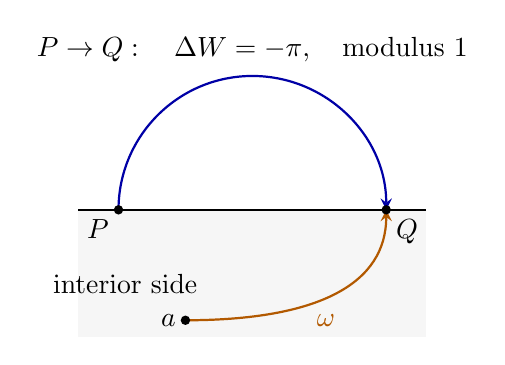
\begin{tikzpicture}[scale=.85,>=stealth]
 \fill[gray!7] (-.6,-1.9) rectangle (4.6,0);
 \draw[thick] (-.6,0)--(4.6,0);
 \draw[blue!65!black,thick,->] (0,0) arc[start angle=180,end angle=0,radius=2];
 \draw[orange!70!black,thick,->] (1,-1.65) .. controls (3,-1.65) and (4,-1.1) .. (4,0);
 \fill (0,0) circle(2pt) node[below left] {$P$};
 \fill (4,0) circle(2pt) node[below right] {$Q$};
 \fill (1,-1.65) circle(2pt) node[left] {$a$};
 \node at (2,2.4) {$P\to Q:\quad\Delta W=-\pi,\quad\text{modulus }1$};
 \node[orange!70!black] at (3.1,-1.65) {$\omega$};
 \node at (.1,-1.1) {interior side};
\end{tikzpicture}
\caption{Local orientation at the target support, rotated to horizontal.
The blue semicircle is a formal exterior connection, not an added lattice
path. The orange path arrives at $Q$ from the interior; its continuation
through the arc uses the reverse orientation. The schematic suppresses
the source support and the lattice.}\label{c:fig:arc}
\end{figure}

\subsection{Removing the exceptional mass}\label{c:tilted-exceptional}
The bound for each individual kernel is now available. Apply the same
comparison to the exceptional set left by the prefix construction.
The same absolute comparison holds with the two left integrals restricted to exceptional paths and the right error still \(C R^{-1/4}(K_Q+K_P)\), with \(C\) independent of \(q\le cR\). To see this, subtract the comparison (in signed-difference form with its error) in \(W'\), starting at \(a'\), integrated over small prefixes. Its right error costs at most the same amount by the prefix injection. And the difference of the two \(f\) factors for a central path and full constructed path costs only \(O(R^{-1/4})\) each, since central completions in the sum stay beyond the prefix cut and avoid the prefix too, and any discarded full-domain completions must reach that cut from clearance of order \(R\). The constants are uniform by smallness of the prefixes.



Fix \(q\) of order \(\rho R\) for small fixed \(\rho>0\), and put
\[
 e_R=R^{1/4}\sum_U E_U\longrightarrow0.
\]
Let \(I_R(q)\) be the sum over the order-\(q\) choices of \(P\) of
\(\int_{a\to P,\,\mathrm{exceptional}}f_W(Q;\omega)\).
To control its possibly singular weight, fix \(0<\delta<1/2\).
Paths with \(\operatorname{dist}(Q,\omega)\ge\delta q\) contribute at
most \(C(\delta q)^{-1/4}\sum_P E_P\), by
\eqref{c:tilted-completion-bounds}. For the remaining paths, discard
the exceptional restriction and sum
\eqref{c:tilted-visit-bound} over dyadic distance bins below \(\delta q\).
The exponent \(3/8-1/4=1/8\) is positive, so, including the final
bounded-distance bin, for \(R\) sufficiently large at fixed
\(\rho,\delta\) this gives
\[
 I_R(q)\le C R^{-1/4}q^{-1/4}
       \bigl(\delta^{-1/4}e_R+\delta^{1/8}\bigr).
\]
First let \(R\to\infty\) at fixed \(\rho,\delta\), then let
\(\delta\downarrow0\). Thus \(I_R(q)=o(R^{-1/4}q^{-1/4})\) for
each fixed \(\rho\). Averaging the exceptional comparison over its
order-\(q\) ports, using the lower bound in
\eqref{c:tilted-completion-bounds} and the individual kernel upper
bound, now yields
\[
 q^{-1/4} E_Q \le o(R^{-1/4}q^{-5/4})+C R^{-1/4} R^{-5/4}.
\]
Here the little-oh may depend on \(\rho\), but the comparison error
constant \(C\) does not. In particular
\[
 \limsup_{R\to\infty}R^{5/4}E_Q\le C\rho^{1/4}.
\]
Letting \(\rho\downarrow0\) proves \(E_Q=o(R^{-5/4})\).



\subsection{The prescribed length law}
Finally count lengths violating either power bound
\(R^{4/3\pm\epsilon}\). Up to mass \(o(R^{-5/4})\), the prefix
construction applies at the prescribed \(Q\). Under the iid law its
prefix length has exponent
\[
 \frac{3/4-\eta}{9/16}=\frac43-\frac{16\eta}{9}
\]
in probability. On small prefixes the center factor is at most
\(CR^{-5/4}\), uniformly in their displacements. Therefore an iid
event of probability \(o(1)\) contributes constructed mass
\(o(R^{-5/4})\), without asserting independence after fixing \(Q\).
Choose \(\eta<9\epsilon/16\). This proves the short-length bound
and also makes prefixes longer than \(\frac12R^{4/3+\epsilon}\)
negligible.

For the appended chord, any specific prefix displacement costs
\(O(k^{-8/3})\) by Proposition~\ref{c:planar-atoms}. Align all new
wedges by lattice translations \(\tau_w\); their apex intersections
are triangular lattice vertices. In the common wedge the endpoints are
\[
 x_w=a+w+\tau_w,\qquad y_w=Q+\tau_w,
 \qquad w=(x_w-y_w)-(a-Q).
\]
Thus each endpoint pair determines its prefix displacement. Since the
angles are fixed and \(|w|=O(R)\) for small prefixes, the apex shift
\(\tau_w\) is also \(O(R)\). In particular there are only \(O(R)\)
possible aligned source ports, all at distance \(O(R)\) from the apex.

We may now sum freely over the endpoint pairs. For appended chords
of diameter above \(S_*=R^{1+\lambda}\), the one-source diameter
bound and the number of sources give \(CRS_*^{-1/4}\).
All smaller-diameter chords lie in a common convex pure truncation of
diameter \(O(S_*)\). The all-endpoint length-mass bound there shows
that those of length above \(\frac12R^{4/3+\epsilon}\) have total mass
at most \(CR^{-4/3-\epsilon}S_*^{25/12+o(1)}\).
Multiplying these two estimates by \(k^{-8/3}\), respectively, gives
\[
 CR^{-5/4-\lambda/4+8\eta/3},\qquad
 R^{-5/4-\epsilon+25\lambda/12+8\eta/3+o(1)}.
\]
Choose first \(\lambda>0\) so that \(25\lambda/12<\epsilon\), then
\(\eta>0\) sufficiently small that both exponents are strictly below
\(-5/4\), while retaining \(\eta<9\epsilon/16\). Both appended-chord
exceptions are consequently \(o(R^{-5/4})\).



Restriction to a hexagon in Theorem~\ref{c:main} can only decrease
these absolute exceptional masses. Its own normalizer is at least
\(cR^{-5/4}\), by Proposition~\ref{c:connectors} and the endpoint
clearances. Dividing proves that both tails vanish in probability
in the restricted domain as well as in the full wedge.

This proves Theorem~\ref{c:tilted-law}. Together with
Theorem~\ref{c:same-side-law} and Theorem~\ref{c:parallel}, it proves
Theorem~\ref{c:main}: the two side supports are identical, parallel, or
nonparallel, and the connector lower bound supplies the normalizer in
each finite hexagon.

\section{Mean length of a prescribed half-plane arch}\label{c:mean}
The same-side probability theorem does not control mean length.
We give a separate marked-arm proof, whose length-weighted contributions
are summable over arch heights at each prescribed gap.
It uses the calibrated finite method and its renewal consequences.

\begin{theorem}[Every-gap half-plane mean length]\label{c:arch-mean}
For two half-plane boundary ports separated by each integer $g\to\infty$,
the probability law $\kappa^{L(\gamma)}/K_g$ satisfies
\[
 L(\gamma)=g^{4/3+o(1)}\quad\hbox{in probability},\qquad
 \mathbb E L(\gamma)=g^{4/3+o(1)}.
\]
\end{theorem}
The finite calibrated estimates in \cite[Theorem 1.2 and Proposition 11.1]{Calibrated} give
$B_h\asymp h^{-1/4}$, $K_g\asymp g^{-5/4}$ with its lower bound
retained at diameter at most $Ag$ for fixed $A$, an exponential lateral
cutoff for a fixed-height strip, and total chord length mass at most
$CR^{25/12}$ in a convex box of size $R$. Their precise confined
length window is not replaced by a pointwise endpoint estimate here.
The probability inputs below are derived from this finite package
in \cite[Proposition 4.1, Lemma 4.2, Lemmas 7.2 and 7.4,
Section 7.3, and Theorem 7.1]{Renewal}.
Proposition 4.1 and Lemma 4.2 give the opening height, diameter,
and length-deficit estimates; Lemma 7.2 gives the atom bounds;
Lemma 7.4 and Section 7.3 give the censored survival test and its
shared-turn application; Theorem 7.1 gives the absolute short-path bound.

\begin{proposition}[Calibrated renewal inputs]\label{c:calibrated-inputs}
For the port-rooted irreducible law, write $Y,Z,L,D$ for integral height,
lateral displacement, length and diameter. Then $2Z$ is integral,
$\Pr(D>r)\le Cr^{-3/4}$,
$1-\mathbb E e^{-tY}\asymp t^{3/4}$, and
$1-\mathbb E e^{-tL}=t^{9/16+o(1)}$. In addition:
\begin{enumerate}
\item[(i)] For $k$ independent whole pieces,
$\sup_j\Pr(S_Y(k)=j)\le Ck^{-4/3}$ and
$\sup_w\Pr(S_{(Y,Z)}(k)=w)\le Ck^{-8/3}$.
The off-axis bridge construction gives positive mass in directional
windows; all atoms use the actual lattice.
\item[(ii)] Start two independent sequences at the same bottom port
through the same first center $v$. Retain completed pieces at heights
strictly below $s$, excluding the first piece reaching or passing $s$.
Fix left and right roles. At every pair of renewal levels
$0<d_1<d_2<s$ from the left and right histories respectively, require
that the prefixes be disjoint after $v$, leave on opposite sides of $v$,
and that every right-prefix crossing at $d_1$ lie strictly right of the
left terminal coordinate. The probability of all these requirements is
at most $C_\eta(1+s)^{-3/4+\eta}$ for each $\eta>0$.
At a shared turn this applies with $s=1$ vacuously, or with $s$
sufficiently below both adjacent arm heights that distant endpoint
adjustments do not affect the tests. For the two arms used below, extending both to the same top port
duplicates just their highest center. The resulting factor of $\kappa$
is absorbed by an absolute constant; no shape-dependent trimming is
used in this application.
\item[(iii)] For every sufficiently small fixed $\xi>0$, some $c,C>0$
give the absolute critical mass estimate
\[
 \sum_{\substack{\omega\text{ rooted at a fixed center}\\
 R\le\diam\omega\le2R,\ L(\omega)\le R^{4/3-\xi}}}
 \kappa^{L(\omega)}\le C e^{-R^c}.
\]
\end{enumerate}
\end{proposition}

\subsection{The two arms and the dyadic target}
Split an arch at a chosen highest vertex. Its two real incident edges go
downwards. Extending both arms to the directly adjacent top wall port
makes them strict downward bridges, duplicating just that vertex. Their
critical product weight therefore differs from the arch weight by a
fixed factor. We count the two shapes from a reference top port, impose
equal heights and transverse displacement difference $g$, and translate
the first bottom endpoint to its prescribed position. This entails no
additional placement sum.

The two ends of this decomposition impose different constraints. At the
top the arms share a turn, so Proposition~\ref{c:calibrated-inputs}(ii)
applies. At the bottom they start at distinct ports a distance $g$ apart;
we will prove a separate weak-order estimate there. To sum length, mark
one irreducible on one arm with its length, and reserve independent
pieces away from both ends and the mark to match height and displacement.
Adding the two choices of rewarded arm bounds the full length weight.

Put $d_*=4/3$ and $a=3/4$. For a dyadic scale $H$, let
\[
 \mathcal M_g(H)=
 \sum_{\substack{\gamma:\,0\to g\text{ a half-plane arch}\\
                  H\le h(\gamma)<2H}}
       L(\gamma)\kappa^{L(\gamma)},
\]
where $h(\gamma)$ is the integral height of the adjacent top wall just
described. The target estimate is
\begin{equation}\label{c:arch-dyadic-target}
 \mathcal M_g(H)\le C_\eta g^{1/4}H^{d_*-2a+O(\eta)}
 \qquad\bigl(H\ge g/\log^2g\bigr).
\end{equation}
The smaller height scales will be negligible by strip confinement.
Since $d_*-2a=-1/6$, summing this bound for sufficiently small $\eta$
gives total length mass $g^{1/12+o(1)}$. Division by
$K_g\gtrsim g^{-5/4}$ then gives the required mean upper bound.

\subsection{A local truncated reward}
The first ingredient bounds the cost of the piece carrying the length
weight.
\begin{lemma}[Truncated length reward]\label{c:truncated-reward}
For the strict irreducible law, as $H\to\infty$,
\[
 \mathbb E[L; Y\le 2H]\le H^{d_*-a+o(1)} .
\]
\end{lemma}
\begin{proof}
Write $\mathcal L_h$ for the total length-weighted mass of strict bridges
of height $h$ from one fixed port, with terminal port summed. Insert a
marked irreducible of height at most $2H$ between two arbitrary strict
bridges of heights at most $H$. Unique irreducible factorization gives
\[
 \left(\sum_{0\le u\le H}B_u\right)^2
       \mathbb E[L;Y\le2H]
 \le \sum_{0\le h\le4H}\mathcal L_h.
\]
Indeed the same output can have several eligible marked pieces, but
their lengths sum to at most its full length. The bridge sum on the left
is of order $H^a$.

For height $h$, restrict first to diameter at most $h\log^2h$. Translate
the source to order $h$ positions and apply the calibrated convex-box
length bound in a box of size $O(h\log^2h)$. This gives
$\mathcal L_h\le h^{13/12+o(1)}$ for the restricted bridges. The larger
diameter tail is negligible by the exponential strip cutoff and the
area bound on length. Bounded strip heights also have exponential
diameter tails: extend them a fixed amount to a sufficiently large
fixed height. Consequently
\[
 \sum_{h\le4H}\mathcal L_h\le H^{a+d_*+o(1)}.
\]
The insertion inequality now proves the claim.
\end{proof}

\subsection{Survival of the order at separated bottom ports}
The shared-turn estimate does not apply at two different starting ports.
We therefore prove the separate weak-order estimate required at the
bottom ends of the arch. This estimate uses the calibrated finite inputs
throughout, independently of the off-axis construction in
Section~\ref{c:same-side}.

\begin{lemma}[Weak order from separated ports]\label{c:bottom-survival}
Start two independent upward irreducible sequences at bottom ports a
distance $g\ge1$ apart, assigning left and right roles by their starts.
Let $\Pi_g(S)$ be the probability that their horizontal endpoint order
is preserved weakly at every common renewal height strictly below $S$.
For $S\ge2$,
\[
 \Pi_g(S)\le C(g/S)^{1/4}\sqrt{\log(2+S)}.
\]
\end{lemma}
\begin{proof}
Their strictly positive common renewal levels themselves form renewals;
write $(T,W)$ for one step, recording height and the signed change of
separation. Pairs reaching the same height split there freely. Their
renewal mass at $j$ is $V_j=B_j^2\asymp(1+j)^{-1/2}$, so the first common
return has total mass one and the pairs restart independently.
Write $b=1/2$. The transform gives
$1-\mathbb E e^{-T/r}\asymp r^{-b}$. Exchanging the two sequences preserves
the joint law of $(T,W)$ and replaces $W$ by $-W$; hence height damping
also preserves displacement symmetry. We first establish
\[
 \Pr(|W|>r)\le C r^{-b},\qquad
 \mathbb E\min(1,|W|/r)\gtrsim r^{-b}.
\]
Pairs in a height bin around \(c_0 r\), with \(c_0\) small, carry summed mass \(\gtrsim r^b\) within individual diameter \(r/3\) by tightness, hence with all \(W\) increments bounded by \(r\). Bounding this by the restricted renewal sum proves the first claim. For the second take integral height \(h\asymp r\). We need strict bridges of height $h$ with endpoint displacement of a fixed nonzero sign and size at least $ch$, each of total mass $\gtrsim h^{-1/4}$. The half-plane continuation in \cite[Section~11, Recoverable half-plane growth]{Calibrated} uses two pure inward normals with dot product $1/2$. For each fixed sufficiently small transverse tolerance, it continues from initial scale $r$ to the exact wall of the second normal at distance $S\ge Kr$, with its terminal port free. Its mass is at least $cS^{-1/4}(S/r)^{-C}$ and diameter at most $C'S$. All centers stay after the initial wall and before the terminal wall, the continuation has the prescribed relative transverse tolerance, and its joining cuts are recoverable. The constants and lower threshold for $r$ may depend on that tolerance.

Apply it first with normals $y,u$ at angle $\pi/3$, initial scale $c_*h$,
and each exact $u$-wall whose level lies in
$[(2-2\delta_*)h,(2-\delta_*)h]$, always summing its terminal ports.
For the later continuation with normals $u,y$, fix in advance a small
transverse tolerance and a sufficiently small initial-scale fraction
compatible with its target-to-initial-scale requirement. Its diameter
constant is then fixed independently of $\delta_*$. Choose $\delta_*$
small in terms of that constant, and then choose the first continuation's
tolerance and $c_*$ sufficiently smaller, also satisfying its required
scale ratio.

The first continuation gains $y$-height with slope $1/2$, so it stays in
$0<y<h$, ends with remaining height between $\delta_*h/4$ and
$2\delta_*h$, and has lateral displacement at least $ch$. Each target
wall has mass $\gtrsim h^{-1/4}$ because all scale ratios are fixed.
Extract the prefix at the lowest qualifying singly crossed $u$-cut in
this bin, using these confinement and terminal-position tests. The mass
summed over target levels is $\gtrsim h^{3/4}$, whereas all suffixes after
a given prefix cost at most $\sum_{j\le Ch}B_j\le Ch^{3/4}$. Distinct
prefixes therefore have mass $\gtrsim1$.

From each prefix apply the $u,y$ continuation with the preselected
tolerance and initial-scale fraction to reach the wall $y=h$ exactly,
again with terminal port free. It stays beyond the joining $u$-cut,
has diameter $O(\delta_*h)$ and mass $\gtrsim h^{-1/4}$. By the choice
of $\delta_*$, it preserves the nonzero lateral displacement and avoids
$y=0$. The joining cut is recovered by its first-qualifying rule. This
proves the asserted strict-bridge mass within the calibrated method.

Reflect the construction for the second bridge. The critical product mass with total transverse difference $\ge ch$ in absolute value is therefore $\gtrsim h^{-1/2}=h^{b-1}$. Bound using subadditivity of \(\min(1,|\cdot|/r)\) over common steps and renewal insertions, costing at most \(\max_{s\le h}\sum_{i+j=s}V_i V_j\) (bounded) times the asserted expectation. This proves the claim. As in the local bounds before (by tail truncation and symmetrization) these imply \(\Pr(c r\le |W|\le r)\gtrsim r^{-b}\) and \(1-|\phi_W(u)|^2\gtrsim |u|^b\) near zero for the characteristic function. Thus independent sums of \(k\) such increments have atoms \(\le C k^{-1/b}\), by lattice Fourier inversion (nonconstant support on a discrete grid).

\paragraph{Counting near-minimum times.}
The distinction between weak and strict survival for lattice increments
is essential; compare \cite[Section 2.2]{Vysotsky2014}. We use the
following direct factorization, which counts all near-minimum times.
Kill at an independent exponential height $E$ of mean $S$. The transverse
walk has symmetric subprobability step kernel
\[
 Q_S(w)=\mathbb E[e^{-T/S};W=w],\qquad
 q_0=1-\sum_wQ_S(w)\asymp S^{-b}.
\]
Let $p$ be its probability of having all partial sums at least $-g$
before death. Write $N_g$ for the number of indices, including time zero,
lying within
$g$ of its global minimum. Then $\mathbb E N_g=p^2/q_0$. Here is a count that
also handles ties. If $a_j(g)$ is the subprobability mass of $j$ steps
whose every partial sum is at least $-g$, then
$p=q_0\sum_{j\ge0}a_j(g)$. At a candidate time with $i$ steps before
it and $j$ after it, reverse and negate the past increments. Symmetry
and independence give mass $q_0a_i(g)a_j(g)$ for the candidate to lie
within $g$ of the minimum. Summing in $i,j$ gives $p^2/q_0$.
Every qualifying candidate is counted; no unique minimum is selected.

\paragraph{Bounding the occupation count.}
The killed kernel is dominated by the original displacement law, including
after convolution:
\[
 Q_S^{*k}(w)\le\Pr(W_1+\cdots+W_k=w).
\]
Thus the atom estimate above bounds the expected number $L_A$ of visits
to any interval $A$ of width $2g$, uniformly in the starting position, by
\[
 \mathbb E L_A\le 1+\sum_{k\ge1}\min\{1,Cgk^{-1/b}\}
 \le Cg^b.
\]
Markov's inequality and restarting after successive visit-count thresholds
give an exponential tail for $L_A$ at scale $g^b$. Anchor an interval of
radius $g$ at each alive index in turn and count its future visits. The
earliest near-minimum index captures all $N_g$ near-minimum visits in its
interval. We do not condition at that retrospectively chosen index:
instead union bound over all indices, whose survival probabilities sum to
$1/q_0$. Consequently
\[
 \Pr(N_g\ge t)\le
 \min\{1,(C/q_0)e^{-ct/g^b}\},\qquad
 \mathbb E N_g\le Cg^b\log(2+1/q_0).
\]
Together with the factorization this bounds $p$ by
$C(g/S)^{b/2}\sqrt{\log(2+S)}$.

Finally, preserving weak order below $S$ also preserves it below $E$ on
$\{E<S\}$. Independence of $E$ from the original sequences gives
\[
 (1-e^{-1})\Pi_g(S)\le p.
\]
Since $b/2=1/4$, this proves the lemma.
\end{proof}

\subsection{Summing the marked-arm decomposition}
\begin{proof}[Proof of Theorem~\ref{c:arch-mean}]
We now have the two different survival tests needed for an arch: the
shared-turn test at its top and Lemma~\ref{c:bottom-survival} at its bottom.
Write $b=1/2$, as in the proof of that lemma.
Use the two-arm decomposition above, whose actual arms are disjoint after
the turn. We will prove \eqref{c:arch-dyadic-target} by allocating independent
groups of pieces to these tests, the reward, and the two-coordinate match.

Use dyads \(H\le h<2H\). Those \(H<g/\log^2 g\) contribute negligibly by exponential strip aspect since one bridge has diameter of order at least \(g\). On remaining dyads diameters above \(C H\log^2 H\) cost \(O_A(H^{-A})\) for arbitrary fixed \(A\), still by strip aspect (sum bridge products at each height, also with lengths using area). Thus in discards with superpolynomial accuracy we may pay a polynomial bound for lengths.

Let \(k_i\) be the two irreducible counts, in dyads at scales \(K_i\), \(K=\max K_i\). Treat their bridge masses at specified counts as product iid laws. Discard \(k_i>H^{a+\eta}\) by height damping, with \(\eta>0\) arbitrarily small fixed (\(k_i\le2H\)). Expand the length weight by marking one piece on its arm. On the other arm also mark a large height jump \(>H^{1-\eta/(2a)}\) (upper bound by counting choices), if \(k_i\le H^{a-\eta}\); without one the height requirement costs superpolynomially little, by exponential weighting at the inverse cutoff on the truncated jumps, using \(\Pr(Y>t)\le C t^{-a}\). For larger count on that arm just designate a middle index instead.

Sort the index distances (counting from 1) of each designated piece from the top and bottom ends into dyadic scales \(I_i,J_i\) respectively. Thus \(\max(I_i,J_i)\asymp K_i\). The sum of index choices and the associated length or large-jump costs have budget, on the two sides combined,
\[
 C_\eta H^{d_*-2a+O(\eta)}
       \prod_{i=1}^2\min(I_i,J_i).
\]
Indeed for a given length piece use Lemma~\ref{c:truncated-reward}; the jump costs \(C H^{-a+O(\eta)}\), and the number of choices on each side is at most a constant times its smaller distance scale. In the middle-index case \(\min(I_i,J_i)H^{-a+\eta}\gtrsim1\) already.

Put $I=\min I_i$ and $J=\min J_i$. The following deterministic allocation makes all uses of independence explicit. Let $r_i$ be the designated index on arm $i$, whose total count is $k_i$, and write
\[
 u_i=r_i-1,\quad v_i=k_i-r_i,\quad
 u=\min_i u_i,\quad v=\min_i v_i.
\]
Take the first $\lfloor u/16\rfloor$ pieces of each arm for the top test and the last $\lfloor v/16\rfloor$ for the bottom test. Neither block contains a designated piece. They are disjoint since $u+v\le k_i-1$ for both arms. On an arm with maximal count $k_{\max}$, at least $15k_{\max}/16-1$ indices remain after these blocks and its designated piece are removed. Reserve the first $\lfloor k_{\max}/4\rfloor$ of these unused indices in their original order for the planar atom; condition on all remaining unreserved draws. The reserved draws need not be consecutive: their displacements still add and they remain independent with the original law.

If $u<16$, the top distance scale $I$ is bounded, so we omit that test and bound its probability by one; this changes the displayed cost below only by a constant. The same holds for $v<16$ and $J$. Otherwise the two testing blocks have orders $I$ and $J$. Bounded $k_{\max}$ is absorbed into constants in the atom bound. This allocation therefore covers marks next to endpoints, unequal arm lengths, and both possible designations. The factors to be multiplied are summarized here; $p'=b/(2a)=1/3$, $m_i=\min(I_i,J_i)$, and the displayed powers of $H$ allow fixed multiples of $\eta$.
\begin{center}
\begin{tabular}{@{}lll@{}}
\toprule
Piece group & Role & Upper cost \\
\midrule
Top blocks on both arms & Shared-turn order & $I^{-1}H^{O(\eta)}$ \\
Designated pieces and indices & Reward and other-arm mark & $H^{d_*-2a+O(\eta)}m_1m_2$ \\
Reserved larger-arm indices & Two-coordinate match & $K^{-2/a}$ \\
Bottom blocks on both arms & Separated-port weak order & $g^{b/2}J^{-p'}H^{O(\eta)}$ \\
\bottomrule
\end{tabular}
\end{center}
The second row includes the designated-index counting allowance. For a large-jump mark this is the actual sum of index choices. In the deterministic middle-index case its cost one is bounded by $m_iH^{-a+\eta}\gtrsim1$ on that arm, so the same combined budget applies; the factor $H^{-a+\eta}$ is not a probability bound on that unconditioned piece. Choices of total counts contribute at most $CK_1K_2$ separately.

With \(S_I=I^{1/a}H^{-C_0\eta}\) for fixed sufficiently large \(C_0\), this many pieces reach height \(S_I\) except with superpolynomial error by height damping if \(S_I\ge2\); similarly at \(S_J=J^{1/a}H^{-C_0\eta}\). Both thresholds are far below \(h\). On valid arms we thus impose Proposition~\ref{c:calibrated-inputs}(ii) up to \(S_I\) (rounded down), by the shared-turn crosscut argument in \cite[Section 7.3]{Renewal}, with the common top-port convention stated in Proposition~\ref{c:calibrated-inputs}(ii), at probability cost \(\le C_\eta I^{-1}H^{O(\eta)}\), allowing roles. At the other end impose weak order at the common cuts below \(S_J\) at cost \(\le C g^{b/2}J^{-b/(2a)}H^{O(\eta)}\), since the two disjoint prefixes to a common cut are strip crosscuts. For thresholds \(<2\) the corresponding upper costs with enlarged \(O(\eta)\) need no test. Reversed shapes are again iid by bridge symmetry, tested as if placed at the prescribed two bottom ports (actual relative placement upon imposing the increment equalities); these tests therefore do not consume information from the middle increments.



In addition the required exact height equality and transverse difference together cost \(\le C K^{-2/a}\) by the local estimate on \((Y,Z)\), reserving order \(K\) other draws of the larger count side independently of both tests and the marks (adjust constant for bounded \(K\)). Including at most \(C K_1 K_2\) pairs of counts, all count-scale factors cancel: writing \(p'=b/(2a)=1/3\),
\[
 K_1K_2 K^{-2/a}\prod_i\min(I_i,J_i)\, I^{-1}J^{-p'}
 \le C K^{-2/a}\max(I_1,I_2)\max(J_1,J_2)J^{1-p'}
 \le C.
\]
Thus including polylogarithmic bin sums proves \eqref{c:arch-dyadic-target}.
Since $d_*-2a<0$, summation and free choice of $\eta$ give total length
mass at most $g^{1/12+o(1)}$ for both arms.

The length-weighted bound is $K_g\mathbb E L\le g^{1/12+o(1)}$.
Dividing by $K_g\ge cg^{-5/4}$ proves the mean upper bound and the
long-length probability bound by Markov's inequality. For the lower
probability bound, every arch has diameter at least a fixed multiple of
$g$. Sum Proposition~\ref{c:calibrated-inputs}(iii) over dyadic diameter
bins starting there, taking a slightly smaller exponent slack to absorb
unit and endpoint conventions. The resulting mass is superpolynomially
small compared with $K_g$. Thus the short-length probability tends to
zero; it also gives $\mathbb E L\ge g^{4/3-o(1)}$. This proves
Theorem~\ref{c:arch-mean}.
\end{proof}


The following terminal-summed consequence also appears in the proof of
\cite[Theorem~8.1]{Renewal}. We include its normalization and first-moment
argument to distinguish this confined mixture from the individual-gap law.
\begin{corollary}[Confined macroscopic-gap arches]\label{c:confined-arch-mean}
Fix a half-plane boundary source and choose a sufficiently large fixed
$C$. Give each arch with terminal gap in $[h,2h]$ on one chosen side
and diameter at most $Ch$ its critical weight, then normalize over
this entire set of terminal ports. For every integer $h\to\infty$,
\[
 L(\gamma)=h^{4/3+o(1)}\quad\hbox{in probability},\qquad
 \mathbb E L(\gamma)=h^{4/3+o(1)}.
\]
\end{corollary}
\begin{proof}
The confined pointwise arch lower bound from the calibrated finite
input above, summed over the order $h$ allowed gaps,
gives normalizing mass at least $ch^{-1/4}$ once $C$ is fixed sufficiently
large. For the first moment, translate the source to order $h$ distinct
ports on the same straight side. All translated confined arches fit in
one convex pure box of diameter $O_C(h)$. Distinct sources distinguish
the translated paths, so the calibrated convex-domain length bound
\cite[Proposition 11.1]{Calibrated}, divided by the number of sources,
gives first length mass at most $C_C h^{13/12}$. Division by the
normalizer proves $\mathbb E L\le C_C h^{4/3}$ and the upper probability
tail by Markov's inequality. Every retained arch has diameter at least
a fixed multiple of $h$. Proposition~\ref{c:calibrated-inputs}(iii),
summed over the finitely many diameter bins through $Ch$, makes its
short-length mass superpolynomially small. This proves the lower
probability tail and hence the mean lower bound. The law in this
corollary sums over terminal ports before normalization; it is distinct
from the individual-gap law of Theorem~\ref{c:arch-mean}.
\end{proof}

\section{Endpoint means from polynomial vacuum estimates}\label{c:pvmeans}
We now estimate mean lengths for bridges to prescribed top ports.
The polynomial-vacuum representation controls endpoint variation after
summing over heights. This gives individual-height estimates on one
density-one set, and estimates at every large scale after critical
averaging over even heights.

Let $\mathcal B_h(e)$ be the strict bridges from bottom coordinate $0$
to top coordinate $e\in\mathbb Z+h/2$ at height $h$. Define
\[
 b_h(e)=\sum_{\gamma\in\mathcal B_h(e)}\kappa^{L(\gamma)},\qquad
 b_h^{(L)}(e)=\sum_{\gamma\in\mathcal B_h(e)}L(\gamma)\kappa^{L(\gamma)}.
\]
Thus $b_h=\sum_e b_h(e)=B_h$ and $b_0(e)=\mathbf1_{e=0}$.
\begin{theorem}[One set of density-one heights]\label{c:density-one}
There is one set $G\subseteq\mathbb N$ with
$|G\cap[1,N]|/N\to1$ such that, for every fixed $\delta,\varepsilon>0$,
all sufficiently large $h\in G$ satisfy
\[
 h^{4/3-\varepsilon}\le\frac{b_h^{(L)}(e)}{b_h(e)}
       \le h^{4/3+\varepsilon}
 \quad(e\in\mathbb Z+h/2,\ |e|\le h^{1-\delta}).
\]
\end{theorem}
For $E_H=2\mathbb N\cap[H,2H]$, put
$Z_H=\sum_{h\in E_H}b_h(0)$ and
$M_H=\sum_{h\in E_H}b_h^{(L)}(0)$.
\begin{theorem}[All-even aligned height mixture]\label{c:mixture}
Give each pair $(h,\gamma)$, $h\in E_H$ and
$\gamma\in\mathcal B_h(0)$, probability $\kappa^{L(\gamma)}/Z_H$.
As $H\to\infty$ through all real scales,
\[
 Z_H=H^{-1/4+o(1)},\quad M_H=H^{13/12+o(1)},\quad
 \mathbb E_H L=M_H/Z_H=H^{4/3+o(1)}.
\]
The height marginal is $b_h(0)/Z_H$.
\end{theorem}

The complete finite construction in \cite[Theorem 1.1 and Lemma 8.2]{PolynomialVacuum} gives
$b_h=h^{-1/4+o(1)}$ and
$\sum_e b_h^{(L)}(e)=h^{13/12+o(1)}$, with exponential strip aspect
cutoff. The flat-strip flux identity in \cite[Section 2]{PolynomialVacuum}
is $b_h+\cos(3\pi/8)A_h=1$, where $A_h$ is the raw critical
mass of nontrivial paths that stay inside the height-$h$ strip,
from the fixed bottom source back to the bottom wall,
with the terminal port summed. Let $i$ be its positive-height irreducible
probability, now recording height and transverse displacement. Its array
$i^{(L)}(h,e)$ is the sum of $L(\gamma)\kappa^{L(\gamma)}$ over
irreducibles with those height and displacement coordinates. Convolution
below is in both variables. We use the following exact reward input from
\cite[Proposition 10.1]{Renewal}.

\begin{proposition}[Polynomial-vacuum rewards]\label{c:pv-rewards}
Write $J$ for the height of one piece under $i$, and $L$ for its length.
Set $\alpha=1/4$, $\beta=3/4$, and $d_*=4/3$. Then
\[
 b=\sum_{k\ge0}i^{*k},\qquad b^{(L)}=b*i^{(L)}*b,
\]
\[
 i(J>r)=r^{-\beta+o(1)},\quad
 \mathbb E_i[L;J\le r]\le r^{d_*-\beta+o(1)},\quad
 \mathbb E_i[Le^{-J/r}]=r^{d_*-\beta+o(1)}.
\]
The discounted lower reward is retained on pieces with height at most
$r\log^2r$ and lateral excursion at most $r\log^4r$.
\end{proposition}
Only in this section, $J$ denotes height. We use $\sigma=3/8$ in the winding phases and
$\theta=\pi/8$ in their coefficients.

Reflection makes $b_h(e)$ symmetric in $e$. Heights and offsets both add under concatenation, so the two convolution identities apply to these arrays.
The lower estimates below will hold at every large height. The endpoint
upper estimates will instead be summed over heights; this distinction is
what leads to the two different conclusions of the section.

\subsection{Endpoint variation from two disjoint bridges}
First put \(t_h\) equal to the total critical product mass for two vertex-disjoint bridges with adjacent starts 0,1 in that order. Write \(J_h(u,v)\) for its refinement by ordered endpoints \(u<v\) on top. We claim
\[
 b_h(y)=\sum_{u\le y<v}J_h(u,v).
\]
Indeed take a bridge spectator from 1 to \(y'\) on top and grow an active exit from 0 with phase \(e^{i\sigma W}\), stopping instead just before first contact with the spectator vertices. Take also the balance reversing the roles of 0 and 1 (spectator now from 0 to \(y'\)), multiplied by \(s_0=e^{6i\theta}\), \(\theta=\pi/8\). Revisit pairs cancel; convergence at fixed width in the vertical coordinate (the unbounded horizontal strip) follows by the finite strip exponential lateral cutoff.

At a first contact the three arms from \(0,1,y'\) form a tripod with the central weight included once, with bijections from the contact terms of each balance. The three branches have the same turn phases at the first contact, so their turn phases measured before turning at the center satisfy
\(e^{i\sigma W_{y'}}=e^{i\theta}e^{i\sigma W_0}=e^{-i\theta}e^{i\sigma W_1}\).
Hence the contact terms cancel in this combination (\(s_0=-e^{-2i\theta}\)).

The remaining active arches in the first balance can only go left, separated by the bridge from exits beyond the adjacent port (also no exit at it); in the second only right. Their phases including the combination factor are thus both \(\ell=e^{3i\theta}\). Project by \(X\mapsto \Im(\ell^{-1}X)/\Im(\ell^{-1})\), killing them and giving coefficients \(1,-1\) on the two types of bridge terms. This yields
\[
 b_h(y'-1)-b_h(y')=\sum_{u<y'}J_h(u,y')-\sum_{v>y'}J_h(y',v).
\]
Sum up to \(y'=y\).

Consequently \(\sup_e b_h(e)\le t_h\) and the sum of absolute first differences of \(b_h(\cdot)\) on its coset is at most \(2t_h\). Also
\(t_h\le C(A_{h+1}-A_h)\): reflect so the adjacent ports are on the top of the old strip, join them by the bounded minimal arch in the added one layer, and translate horizontally to put the resulting bottom arch's starting port at the fixed source (use the ordered ends). A strip-exchanging lattice isometry with any needed offset can be used before this translation. Recovery has bounded multiplicity since the crossing ports of the old top line are exactly the two joined ports, adjacent and prescribed before translation. Thus by flat strip flux, for fixed \(0<c_1<c_2<\infty\),
\[
 \sum_{c_1 H\le j\le c_2 H} t_j \le C b_{\lfloor c_1H\rfloor}=H^{-\alpha+o(1)}\quad\text{(as an upper bound)} .
\]

\subsection{A pointwise lower bound at every height}
The variation bound is available only after summing heights. Nevertheless
it will yield a lower bound at each height by averaging internal renewal
cuts. Here is a uniform pointwise \textbf{lower} bound at all large heights for any fixed \(\delta>0\):
\[
 b_h(e)\ \ge\ h^{-1-\alpha-o(1)} \qquad (|e|\le h^{1-\delta},\ e\in\mathbb Z+h/2).
\]
First take even \(h\). For a bridge \(\gamma\in\mathcal B_h(e)\), let
\(N_h(\gamma)\) count the integers \(j\in[h/8,h/7]\) for which all
three levels \(j,2j,h/2+j\) are single-crossing cuts. Put
\(k=h/2-j\). Splitting at those cuts gives four bridges of heights
\(j,j,k,k\), so, with convolution here only in the offset,
\[
 \sum_{\gamma\in\mathcal B_h(e)}N_h(\gamma)\kappa^{L(\gamma)}
 =\sum_{h/8\le j\le h/7}(b_j*b_j*b_k*b_k)(e).
\]
For all but \(o(h)\) of these internal levels \(j\), the summed
variation estimate gives \(t_j\le h^{-1-\alpha+\delta_0/8}\), where
\(\delta_0=\min(\delta,1/2)\). The external height \(h\) remains
arbitrary. Write \(A=b_j(\cdot)*b_k(\cdot)\). Its total is
\(b_j b_k\), concentrated on \(|x|\le Ch\log^2 h\) up to negligible
tails by the exponential horizontal strip bounds; its sup norm and total
variation on its coset are bounded by \(t_j b_k,2t_j b_k\)
respectively. Thus
\[
 \sum_x A(x)A(e-x)
 =\sum_x A(x)A(x-e)\ \ge\ \|A\|_2^2-2|e|t_j^2 b_k^2,
 \qquad
 \|A\|_2^2\ge h^{-1-o(1)}(b_jb_k)^2.
\]
For good \(j\) the subtracted term is negligible. Summing gives first moment at least \(h^{-4\alpha-o(1)}\).

For the second moment, diagonal terms cost at most \(h^{-4\alpha+o(1)}\) in sum (use \(\sup b_j(\cdot)\le t_j\) on one factor). Off-diagonal terms \(j<j'\) are cut up by the union of both triples of levels, yielding endpoint convolution masses of seven bridges: four of heights comparable to \(h\), including \(j\), and three of heights \(\Delta,2\Delta,\Delta\), \(\Delta=j'-j\). Bound pointwise using the sup at \(j\) and total masses for all others. Since \(\sum_{\Delta\le h}b_\Delta^2 b_{2\Delta}\le h^{1-3\alpha+o(1)}\), summation of \(t_j\) gives
\[
 \sum_{\gamma\in\mathcal B_h(e)}N_h(\gamma)^2\kappa^{L(\gamma)}
 \le h^{1-7\alpha+o(1)}.
\]
Weighted Cauchy--Schwarz therefore gives
\[
 b_h(e)\ge
 \frac{\bigl(\sum_{\gamma\in\mathcal B_h(e)}
 N_h(\gamma)\kappa^{L(\gamma)}\bigr)^2}
 {\sum_{\gamma\in\mathcal B_h(e)}
 N_h(\gamma)^2\kappa^{L(\gamma)}}
 \ge h^{-1-\alpha-o(1)}.
\]
Odd heights follow by a bounded one-layer extension from even height
with the appropriate half-step endpoint shift, using a lower-bound
window with a smaller positive \(\delta\).

\subsection{Inserting length between two bridge kernels}
Write \(K=b*b\) in both height and offset. It follows that
\[
 K_h(e)\ge h^{-2\alpha-o(1)} \qquad (|e|\le h^{1-\delta})
\]
again for admissible offsets. Indeed sum over heights \(h/3\le l\le 2h/3\) and offsets \(|x|\le h^{1-\eta}\) of the first factor, for arbitrarily small \(0<\eta<\delta/2\); both factors use the preceding lower bound with sublinear power windows. Send \(\eta\) down. On the upper side we have
\[
 \sum_{j\le 2H}\sup_x K_j(x)\le H^{2\beta-1+o(1)} .
\]
Order the two factor heights by size, larger \(l\) and smaller \(r\). Apart from zero total height use \(\sup b_l(\cdot)\le t_l\) and \(\sum_{r\le l} b_r\le l^{\beta+o(1)}\) (up to constants); summing dyadically gives the bound since \(\beta-\alpha>0\).

The length insertion is exactly \(b^{(L)}=K*i^{(L)}\). Uniformly in the same windows we obtain the pointwise lower bound
\[
 b_h^{(L)}(e)\ge h^{d_*+\beta-2-o(1)}.
\]
In fact take the middle piece from \(i^{(L)}\) with height \(\le m\log^2 m\) and absolute displacement \(\le m\log^4 m\), \(m=h^{1-\varepsilon}\), for small fixed \(\varepsilon>0\). Its available total mass is at least \(m^{d_*-\beta-o(1)}\), by the exponentially height-discounted first moment and tail truncations in Proposition~\ref{c:pv-rewards}. The remaining \(K\) uses height comparable to \(h\). Since \(m\log^4m\le h^{1-\varepsilon/2}\) for large \(h\), its offset still lies in a sublinear power window for each fixed \(\delta,\varepsilon>0\). Use the lower bound for \(K\) and send \(\varepsilon\) to zero. Also
\[
 \sum_{H\le h\le 2H}\sup_e b_h^{(L)}(e)\le H^{d_*+\beta-1+o(1)}
\]
by the upper \(K\) estimate and the truncated \(i^{(L)}\) upper bound up to height \(2H\).

\subsection{One density-one set and the aligned mixture}
Put $U_h=\sup_e b_h(e)$ and $V_h=\sup_e b_h^{(L)}(e)$, with the
suprema over the actual row coset. For dyadic $H$, choose
$\rho_H\to\infty$ with $\rho_H=H^{o(1)}$ so that the two summed
upper bounds give
\[
 \sum_{H\le h<2H}U_h\le\rho_H H^{-\alpha},\qquad
 \sum_{H\le h<2H}V_h\le\rho_H H^{d_*+\beta-1}.
\]
In each such interval retain precisely the heights satisfying
\[
 U_h\le\rho_H^2 H^{-1-\alpha},\qquad
 V_h\le\rho_H^2 H^{d_*+\beta-2},
\]
and let $G$ be the union of the retained heights. At most
$2H/\rho_H=o(H)$ heights are removed from each interval. Summing
over dyadic intervals shows that $G$ has density one. On $G$,
\[
 \sup_e b_h(e)\le h^{-5/4+o(1)},\qquad
 \sup_e b_h^{(L)}(e)\le h^{1/12+o(1)}.
\]
The construction of $G$ uses global endpoint suprema and does not
depend on $\delta$ or $\varepsilon$. For each fixed $\delta>0$, the
all-height lower bounds give, uniformly on its admissible window,
$b_h(e)\ge h^{-5/4-o(1)}$ and
$b_h^{(L)}(e)\ge h^{1/12-o(1)}$. Combining the lower numerator with
the upper denominator, and then the upper numerator with the lower
denominator, yields
\[
 h^{4/3-o(1)}\le\frac{b_h^{(L)}(e)}{b_h(e)}
 \le h^{4/3+o(1)}\qquad(h\in G,\ |e|\le h^{1-\delta}).
\]
This proves Theorem~\ref{c:density-one} with its stated quantifiers.

For completeness, the mixture in Theorem~\ref{c:mixture} follows directly from the estimates before that deletion of heights. At each large even height, the aligned lower bounds are $b_h(0)\ge h^{-5/4-o(1)}$ and $b_h^{(L)}(0)\ge h^{1/12-o(1)}$. Summing over the order $H$ even heights in $[H,2H]$ gives $Z_H\ge H^{-1/4-o(1)}$ and $M_H\ge H^{13/12-o(1)}$. The dyadic sums of the endpoint suprema give the reverse bounds $Z_H\le H^{-1/4+o(1)}$ and $M_H\le H^{13/12+o(1)}$. Their ratio proves the mixture mean at every large scale. No upper estimate at an individual discarded height has been used.

\begin{thebibliography}{99}\bibitem{AlexanderBerger2016}
K.~S. Alexander and Q.~Berger.
Local asymptotics for the first intersection of two independent renewals.
\emph{Electronic Journal of Probability} \textbf{21} (2016), paper 68, 1--20.
\href{https://arxiv.org/abs/1603.05531}{arXiv:1603.05531}.

\bibitem{BeatonEtAl2014}
N.~R. Beaton, M.~Bousquet-M\'elou, J.~de Gier, H.~Duminil-Copin and A.~J. Guttmann.
The critical fugacity for surface adsorption of self-avoiding walks on the
honeycomb lattice is $1+\sqrt2$.
\emph{Communications in Mathematical Physics} \textbf{326} (2014), 727--754.
\href{https://doi.org/10.1007/s00220-014-1896-1}{doi:10.1007/s00220-014-1896-1}.

\bibitem{DuminilCopinSmirnov2012}
H.~Duminil-Copin and S.~Smirnov.
The connective constant of the honeycomb lattice equals $\sqrt{2+\sqrt2}$.
\emph{Annals of Mathematics} \textbf{175} (2012), 1653--1665.
\href{https://doi.org/10.4007/annals.2012.175.3.14}{doi:10.4007/annals.2012.175.3.14}.

\bibitem{DyhrEtAl2011}
B.~Dyhr, M.~Gilbert, T.~Kennedy, G.~F.~Lawler and S.~Passon.
The self-avoiding walk spanning a strip.
\emph{Journal of Statistical Physics} \textbf{144} (2011), 1--22.
\href{https://doi.org/10.1007/s10955-011-0258-z}
{doi:10.1007/s10955-011-0258-z}.
\href{https://arxiv.org/abs/1008.4321}{arXiv:1008.4321}.

\bibitem{Gilbert2015}
M.~J.~Gilbert.
The fixed irreducible bridge ensemble for self-avoiding walks.
\emph{Journal of Statistical Physics} \textbf{159} (2015), 321--335.
\href{https://doi.org/10.1007/s10955-014-1137-1}
{doi:10.1007/s10955-014-1137-1}.

\bibitem{GlazmanManolescu2017}
A.~Glazman and I.~Manolescu.
Self-avoiding walk on $\mathbb Z^2$ with Yang--Baxter weights:
universality of critical fugacity and 2-point function.
\emph{Annales de l'Institut Henri Poincar\'e, Probabilit\'es et Statistiques}
\textbf{56} (2020), 2281--2300.
\href{https://doi.org/10.1214/19-AIHP1024}{doi:10.1214/19-AIHP1024}.

\bibitem{Jaffard1990}
S.~Jaffard.
Propri\'et\'es des matrices ``bien localis\'ees'' pr\`es de leur diagonale
et quelques applications.
\emph{Annales de l'Institut Henri Poincar\'e C, Analyse non lin\'eaire}
\textbf{7} (1990), 461--476.
\href{https://doi.org/10.1016/S0294-1449(16)30287-6}{doi:10.1016/S0294-1449(16)30287-6}.

\bibitem{Kesten1963}
H.~Kesten.
On the number of self-avoiding walks.
\emph{Journal of Mathematical Physics} \textbf{4} (1963), 960--969.
\href{https://doi.org/10.1063/1.1704022}{doi:10.1063/1.1704022}.

\bibitem{KrachunPanagiotis2026}
D.~Krachun and C.~Panagiotis.
Quantitative sub-ballisticity of self-avoiding walk on the hexagonal lattice.
\emph{Annals of Probability} \textbf{54} (2026), 1109--1125.
\href{https://doi.org/10.1214/24-AOP1730}{doi:10.1214/24-AOP1730}.

\bibitem{LawlerSchrammWerner2004}
G.~F.~Lawler, O.~Schramm and W.~Werner.
On the scaling limit of planar self-avoiding walk.
In \emph{Fractal Geometry and Applications: A Jubilee of Beno\^it Mandelbrot},
Part~2, Proceedings of Symposia in Pure Mathematics \textbf{72},
American Mathematical Society, 2004, 339--364.
\href{https://arxiv.org/abs/math/0204277}{arXiv:math/0204277}.

\bibitem{Nienhuis1982}
B.~Nienhuis.
Exact critical point and critical exponents of $O(n)$ models in two dimensions.
\emph{Physical Review Letters} \textbf{49} (1982), 1062--1065.
\href{https://doi.org/10.1103/PhysRevLett.49.1062}{doi:10.1103/PhysRevLett.49.1062}.

\bibitem{Calibrated}
OpenAI.
Cylinder amplitudes and logarithmic bridge-length windows on the honeycomb lattice.
OpenAI Math Release preprint
\href{https://github.com/openai/math/blob/main/preprints/Cylinder-amplitudes-and-logarithmic-bridge-length-windows-on-the-honeycomb-lattice-September-26-2026/main.pdf}{OAI:Cylinder-amplitudes-and-logarithmic-bridge-length-windows-on-the-honeycomb-lattice-September-26-2026},
2026.

\bibitem{DiskTransfer}
OpenAI.
Disk transfer representations and confined bridge mass.
OpenAI Math Release preprint
\href{https://github.com/openai/math/blob/main/preprints/Disk-transfer-representations-and-confined-bridge-mass-September-26-2026/main.pdf}{OAI:Disk-transfer-representations-and-confined-bridge-mass-September-26-2026},
2026.

\bibitem{PolynomialVacuum}
OpenAI.
Polynomial vacuum representations and bridge mass for honeycomb walks.
OpenAI Math Release preprint
\href{https://github.com/openai/math/blob/main/preprints/Polynomial-vacuum-representations-and-bridge-mass-for-honeycomb-walks-September-26-2026/main.pdf}{OAI:Polynomial-vacuum-representations-and-bridge-mass-for-honeycomb-walks-September-26-2026},
2026.

\bibitem{Renewal}
OpenAI.
Renewal and changes of law for critical honeycomb walks.
OpenAI Math Release preprint
\href{https://github.com/openai/math/blob/main/preprints/Renewal-and-changes-of-law-for-critical-honeycomb-walks-September-26-2026/main.pdf}{OAI:Renewal-and-changes-of-law-for-critical-honeycomb-walks-September-26-2026},
2026.

\bibitem{UniformMarked}
OpenAI.
Uniform marked-polygon estimates and sharp finite bridge moments.
OpenAI Math Release preprint
\href{https://github.com/openai/math/blob/main/preprints/Uniform-marked-polygon-estimates-and-sharp-finite-bridge-moments-September-26-2026/main.pdf}{OAI:Uniform-marked-polygon-estimates-and-sharp-finite-bridge-moments-September-26-2026},
2026.

\bibitem{Simon2005Szego}
B.~Simon. The sharp form of the strong Szeg\H{o} theorem.
In \emph{Geometry, Spectral Theory, Groups, and Dynamics},
Contemporary Mathematics \textbf{387}, American Mathematical Society,
2005, 253--275. \href{https://arxiv.org/abs/math/0402110}{arXiv:math/0402110}.

\bibitem{Vysotsky2014}
V.~Vysotsky. Positivity of integrated random walks.
\emph{Annales de l'Institut Henri Poincar\'e, Probabilit\'es et Statistiques}
\textbf{50} (2014), 195--213.
\href{https://doi.org/10.1214/12-AIHP487}{doi:10.1214/12-AIHP487}.
\end{thebibliography}
\end{document}
